% ======================================================================
%  Constrained-worldline brachistochrones in non-stationary spacetimes
%  IOP iopart class -- Classical and Quantum Gravity
% ======================================================================
\documentclass[12pt]{iopart}

% iopart pre-defines \equation*, which clashes with amsmath; free it first
\makeatletter
\expandafter\let\csname equation*\endcsname\relax
\expandafter\let\csname endequation*\endcsname\relax
\makeatother
\usepackage{amsmath}
\usepackage{iopams}
\usepackage{graphicx}
\usepackage{bm}
\usepackage{xcolor}
\usepackage{hyperref}
\hypersetup{colorlinks=true, linkcolor=blue, citecolor=blue, urlcolor=blue}

% all figures collected here as PNG
\graphicspath{{Immagini/}}

% prose placeholder helper
\newcommand{\todo}[1]{{\color{red}\small[[#1]]}}

% shortcuts
\newcommand{\Ehat}{\hat E}
\newcommand{\rp}{r_{+}}
\newcommand{\re}{r_{e}}
\newcommand{\Jc}{J_{c}}
\newcommand{\Af}{A_{\mathrm{freeze}}}
\newcommand{\dd}{\mathrm{d}}

\begin{document}

\title{Constrained-worldline brachistochrones in non-stationary
spacetimes: Kodama rails, closed forms, and plunge inversion}

\author{Iman Rosignoli}
\address{University of Pavia, Pavia, Italy}
\ead{iman.rosignoli01@universitadipavia.it}

\begin{abstract}
We extend the relativistic brachistochrone (fastest-descent
constrained rail curves, Perlick 1991) from stationary to non-stationary
spacetimes. The rail constraint $-u\cdot W=\Ehat$ is an actively controlled
invariant, legitimate via Pontryagin's principle; the selector $W$ follows a
hierarchy Killing $\to$ conformal Killing $\to$ Kodama vector. We treat FLRW
(degenerate base), Vaidya (dynamical black hole, $W=\partial_v$ the Kodama
vector), and Thakurta--Kerr (conformal rotating compact object). Main results:
Kodama energy conservation along the rail; the plunge-radius law and the
absence of a \emph{physical} evaporative inversion (only rotation and the
conformal factor invert); closed-form equatorial separatrices in Weierstrass
functions with Doran continuation through the ergosphere; the trichotomy at
the ergosphere with an analytic cusp theorem; and an existence theorem for the
conformal plunge inversion.
\end{abstract}

\maketitle

{\hypersetup{linkcolor=black}\tableofcontents}


% ======================================================================
\section{Introduction}
\label{sec:intro}
% ----------------------------------------------------------------------
The relativistic brachistochrone---the fastest constrained ``rail'' worldline
between two events---was formulated by Perlick for stationary spacetimes
\cite{Perlick1991,PerlickRayOptics}, where a timelike Killing vector provides
the conserved rail energy. It connects naturally to Fermat's principle and to
optical (Randers--Zermelo--Finsler) geometry
\cite{Kovner1990,Randers1941,GibbonsWerner2008,GibbonsRanders2009,BaoRoblesShen}.
Building on our earlier relativistic-brachistochrone studies---the stationary
Kerr geometry \cite{RosignoliKerr}, the interior Schwarzschild metric
\cite{RosignoliIntSchw}, and Tolman--Oppenheimer--Volkoff stellar interiors
\cite{RosignoliTOV}---we extend the construction to \emph{non-stationary}
spacetimes: FLRW, Vaidya \cite{Vaidya1951}, and Thakurta--Kerr
\cite{Thakurta1981}.
These extensions raise three questions that organize the paper.
\emph{(i) Is the rail constraint legitimate without a Killing vector?} We show it
is: $-u\cdot W=\Ehat$ is an actively controlled invariant, and the fastest
constrained worldline solves a well-posed time-optimal control problem
(Sec.~\ref{sec:principle}) whose control cost measures precisely the missing
symmetry. \emph{(ii) What replaces the conserved energy?} In a spherically
symmetric dynamical spacetime the selector $W$ is the Kodama vector, whose flux
charge is the Misner--Sharp mass; the rail conserves the Kodama energy
identically even though it is \emph{not} Noether-conserved for free fall
(Sec.~\ref{sec:vaidya}). \emph{(iii) Which phenomena are genuinely
non-stationary?} We isolate three: capture by cosmological expansion, the
teleological (future-anticipating) turning point in Vaidya, and the breathing
freezing surface that eats the radius of convergence of the quasi-constants in
Thakurta--Kerr. The three spacetimes form a ladder of increasing structure---%
FLRW (degenerate base), Vaidya (dynamical horizon), Thakurta--Kerr
(rotation $+$ conformal expansion)---treated in
Secs.~\ref{sec:flrw}--\ref{sec:thakurta}; equatorial closed forms and the
plunge-inversion analysis follow in Secs.~\ref{sec:closed}--\ref{sec:bvp}.


% ======================================================================
\section{The controlled-rail principle}
\label{sec:principle}
% ----------------------------------------------------------------------

\subsection{Rail constraint and the indicatrix}
\label{sec:indicatrix}
The rail is a constrained worldline with the invariant
\begin{equation}
    -\,u\cdot W \;=\; \Ehat ,
    \label{eq:rail}
\end{equation}
actively maintained by an ideal (magnetic-type) rail force $f_\mu=Du_\mu/\dd\tau$
with $f\cdot u=0$, so that the rail does no work on the particle.

\paragraph{The ellipse.} Fix an event and a time function adapted to $W$. The
linear constraint~\eqref{eq:rail} fixes the $W$-component of $u$; the mass shell
$u\cdot u=-1$ is a quadric; their intersection, projected onto the physical
velocity plane $(\dd r,\,r\,\dd\varphi)$ per unit selector-time, is an ellipse
\begin{equation}
    \dot x(\theta)=c+R(\theta),\qquad \theta\in[0,2\pi),
    \label{eq:ellipse}
\end{equation}
whose center $c$ is the Zermelo wind (zero for FLRW, ingoing radial for Vaidya,
azimuthal---frame dragging---for Thakurta--Kerr) and whose axes $R$ shrink with
the local speed as the freezing surface is approached (Fig.~\ref{fig:indicatrici}).
Every branch---arrival time $t$, proper time $\tau$, conformal time $\eta$---shares
this \emph{same} indicatrix; the branches differ only in the cost one-form, i.e.\
in which clock measures the elapsed travel time.

\paragraph{Pontryagin reduction.} Minimizing travel time subject
to~\eqref{eq:ellipse} is a time-optimal control problem with control $\theta$.
Since the admissible-velocity set is a smooth strictly convex oval, the maximizer
of $p\cdot\dot x(\theta)$ is unique and Pontryagin's maximum principle
\cite{Pontryagin,Liberzon} delivers the branch Hamiltonian $H(x,p)$ in closed
form (Secs.~\ref{sec:vaidya}--\ref{sec:thakurta}); the convex-oval regularity
makes the vakonomic and d'Alembert formulations coincide, so no Filippov
relaxation is needed. Two structural facts hold throughout: the transversality
condition
\begin{equation}
    H=0 \qquad\text{(free arrival time),}
    \label{eq:transversality}
\end{equation}
and $p_\varphi=J$ conserved (axial symmetry). In the stationary limit $H$ is
autonomous and $H\equiv0$ is a genuine first integral; non-stationarity enters
only through the explicit time dependence $\dd H/\dd(\text{time})=
\partial_{\text{time}}H$, proportional to $m'(v)$ (Vaidya) or $A'(\eta)$
(Thakurta--Kerr).

\paragraph{Cost of control.} Differentiating the invariant along the worldline,
\begin{equation}
    \frac{\dd(-u\cdot W)}{\dd\tau}=-\,u^a u^b\,\nabla_{(a}W_{b)},
    \label{eq:cost}
\end{equation}
which vanishes for \emph{all} $u$ iff $W$ satisfies the Killing equation. When it
does not, the right-hand side is the power the rail force must supply to hold
$\Ehat$ fixed: the control cost equals the failure of the Killing equation, i.e.\
the missing symmetry. This is why the non-stationary rail is legitimate but not
free---$\Ehat$ is controlled, not conserved. The optical reductions of $H$
reproduce the Randers/Zermelo structure
\cite{GibbonsRanders2009,CaponioWind}.

\paragraph{Geometric dictionary.} The indicatrix~\eqref{eq:ellipse} carries two
independent data---its \emph{center} $c=(c_r,c_\varphi)$ (the Zermelo wind) and
the \emph{eccentricity} of its semi-axes (the anisotropy of the local speed,
$a_r\neq a_\varphi$)---and each governs a distinct feature of the
brachistochrones, the same for every branch:
\begin{itemize}\itemsep2pt
\item eccentricity $\neq0$ (a spatial gradient $\partial_r f\neq0$)
$\Rightarrow$ the $t$ and $\tau$ branches split in depth, $n_t/n_\tau=E/f\neq1$;
\item azimuthal offset $c_\varphi\neq0$ (frame dragging)
$\Rightarrow$ rotational plunge inversion becomes possible;
\item radial offset $c_r\neq0$ (a non-stationary wind, $m'\neq0$)
$\Rightarrow$ teleological memory, $p_v\neq0$ along the path;
\item shrinking axes $R\to0$ (local speed $v\to0$) $\Rightarrow$ freezing and
capture.
\end{itemize}
Eccentricity and center offset are \emph{separate} levers: the first switches on
the $t/\tau$ split, the second the inversions. In particular the three branches
\emph{degenerate}---the $t$, $\tau$ and $\eta$ brachistochrones coincide---iff the
indicatrix is, up to a position-independent conformal scale, a rigid centered
circle ($c=0$, $a_r=a_\varphi$, radius depending on the flow parameter alone),
equivalently iff the optical cost ratios $n_t/n_\tau,\,n_t/n_\eta$ are
position-independent. This is exactly spatial homogeneity: FLRW is the unique
such case in our ladder (Sec.~\ref{sec:flrw}), whereas any gradient or wind
breaks it---even the static, non-rotating Schwarzschild ellipse, which is
centered ($c=0$) yet eccentric, already splits $t$ from $\tau$. The indicatrix
shape is thus the organizing thread of the paper: FLRW (circle) $\to$ Vaidya
(radial wind) $\to$ Thakurta--Kerr (angular wind) is a progression of ellipse
deformations, each switching on one further phenomenon.

\begin{figure}[tbp]
    \centering
    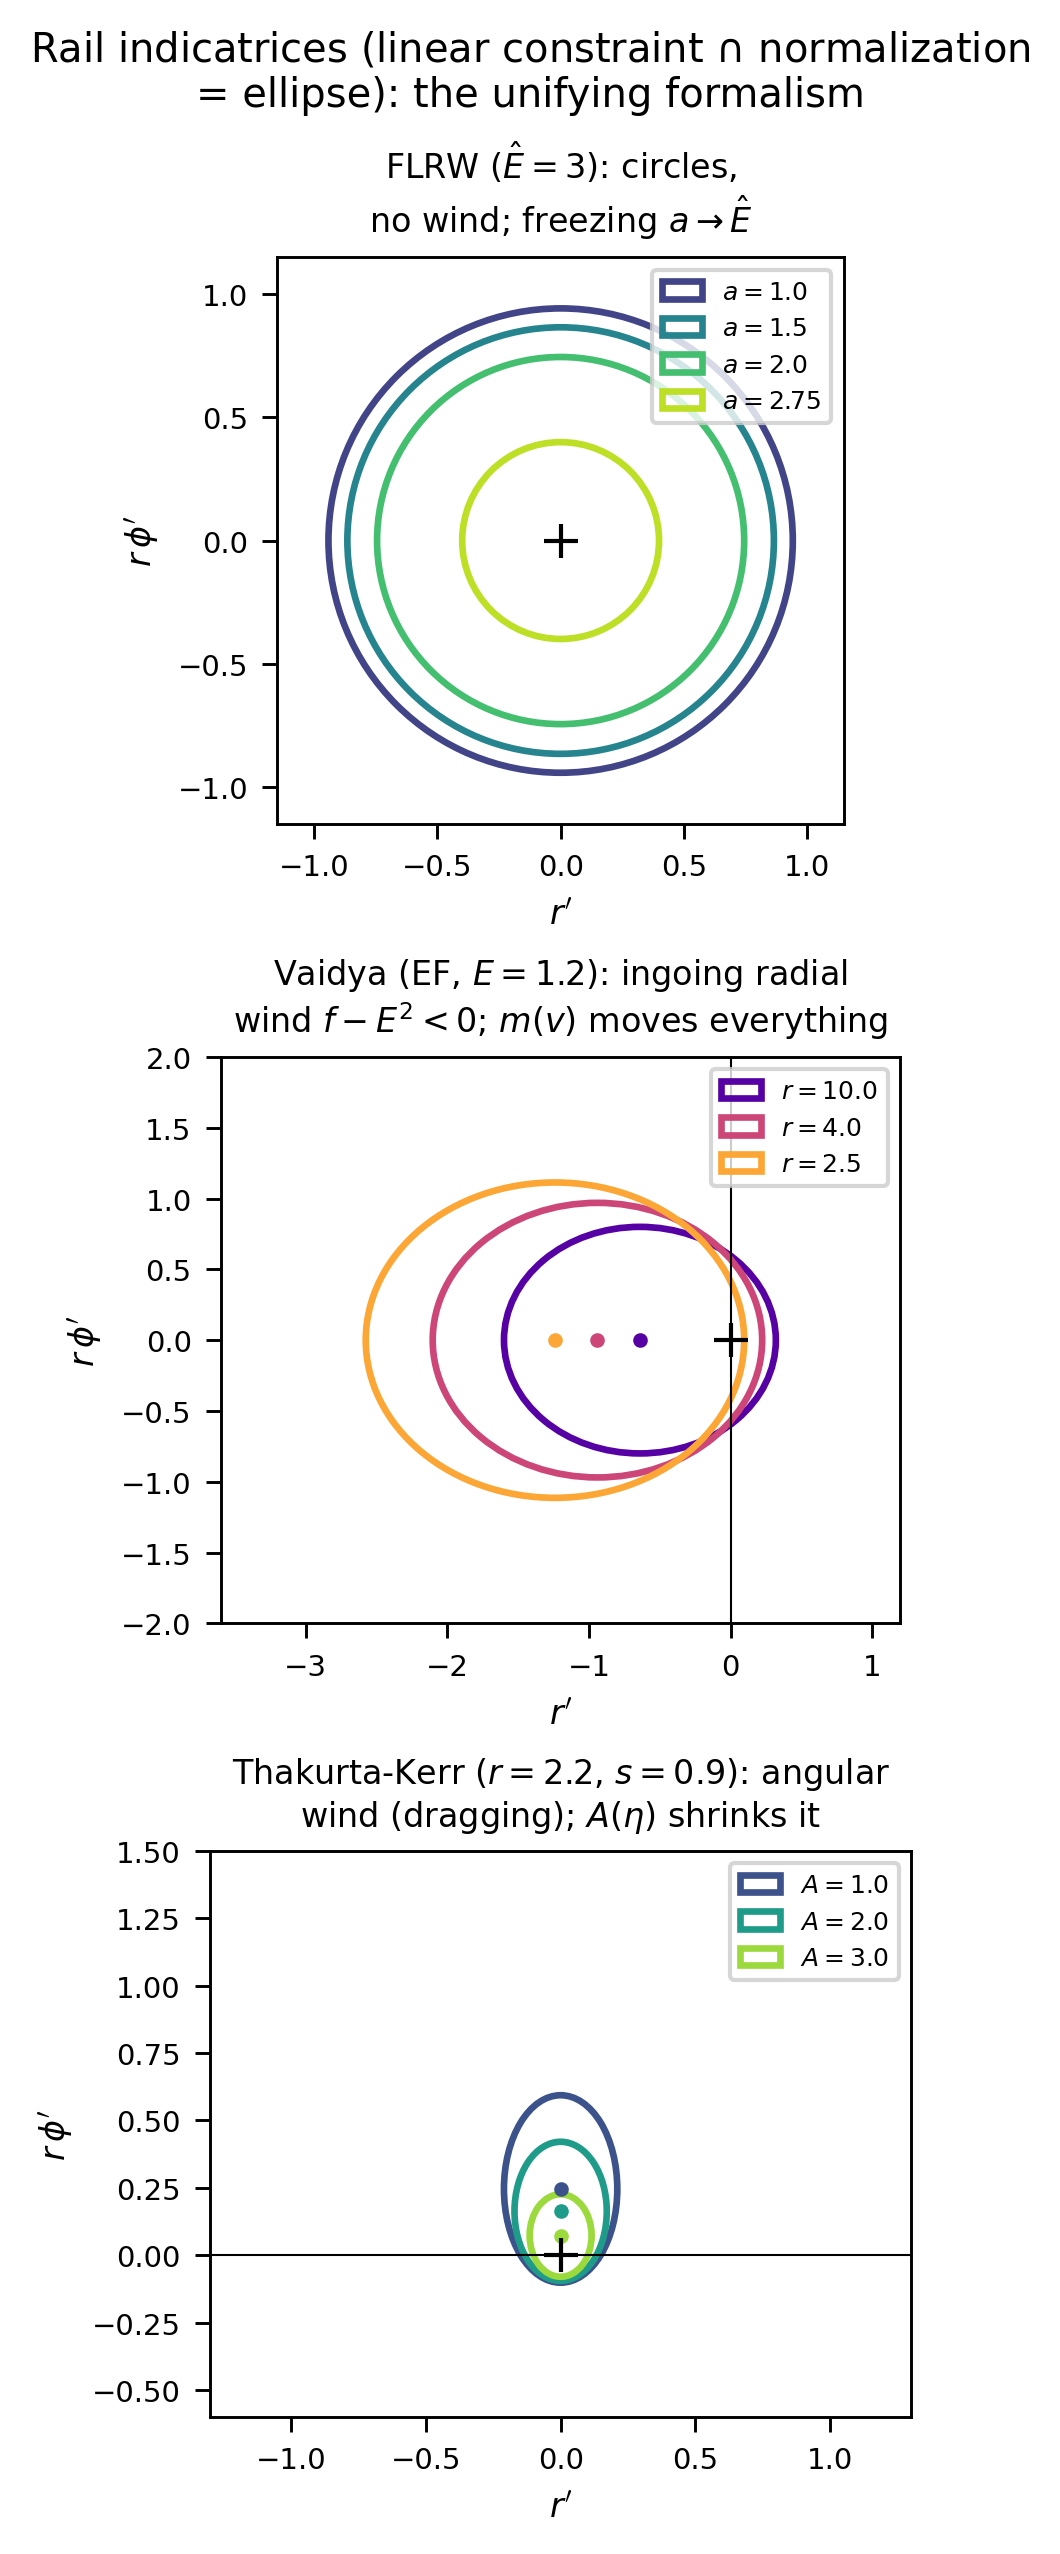
\includegraphics[width=\textwidth,height=0.68\textheight,keepaspectratio]{Immagini/fig_indicatrici.png}
    \caption{Rail indicatrices (linear constraint $\cap$ normalization
    $=$ ellipse): the unifying formalism. FLRW gives shrinking circles (no
    wind, no eccentricity $\Rightarrow$ degenerate branches); Vaidya an ingoing
    radial wind ($f-E^2<0$, driven by $m(v)$ $\Rightarrow$ teleological memory);
    Thakurta--Kerr an angular wind (frame dragging $\Rightarrow$ rotational
    inversion), the ellipse shrinking with $A(\eta)$. Eccentricity switches on
    the $t/\tau$ split, the center offset the inversions.}
    \label{fig:indicatrici}
\end{figure}

\subsection{Selecting $W$: the Killing--CKV--Kodama hierarchy}
\label{sec:whierarchy}
The selector $W$ is fixed by a hierarchy of decreasing symmetry, each level
recovering the previous one in the appropriate limit.

\emph{(a) Killing.} If a timelike Killing vector $\xi$ exists, $W=\xi$ and the
right-hand side of Eq.~\eqref{eq:cost} vanishes identically: $-u\cdot\xi$ is
Noether-conserved and the rail is free. This is Perlick's stationary case
\cite{Perlick1991}.

\emph{(b) Conformal Killing.} If the spacetime is conformally stationary,
$g=\Omega^2\hat g$ with $\hat g$ stationary, the timelike conformal Killing
vector $\partial_\eta$ selects the conformal-time branch; $-u\cdot W$ is exactly
conserved for null rays and controlled up to the conformal factor for massive
rails. FLRW and constant-$A$ Thakurta--Kerr live at this level.

\emph{(c) Kodama.} In a spherically symmetric \emph{dynamical} spacetime with no
Killing or conformal Killing vector, the Kodama vector
$K^a=\varepsilon^{ab}\nabla_b r$ \cite{Kodama1980,Hayward1996} is the canonical
replacement: it is divergence-free (Eq.~\eqref{eq:kodama}), reduces to $\xi$ in
the static limit, and its flux $G^{ab}K_b$ is conserved with charge the
Misner--Sharp mass. Vaidya is the paradigm (Sec.~\ref{sec:kodama-energy}).

\emph{(d) Convention.} Absent even spherical symmetry the Kodama construction
fails and $W$ becomes a declared convention, with no distinguished normalization
of the cost one-form. Levels (a)--(c) are what make the non-stationary rail
canonical rather than arbitrary.


% ======================================================================
\section{FLRW: the degenerate base case}
\label{sec:flrw}
% ----------------------------------------------------------------------
For spatially flat FLRW, $g=a(\eta)^2\eta_{\rm Mink}$, the rail uses the
conformal Killing vector $\partial_\eta$; the local speed is
\begin{equation}
    v(\eta)=\sqrt{1-a(\eta)^2/\Ehat^{2}},
    \label{eq:flrwspeed}
\end{equation}
vanishing at the freezing barrier $a=\Ehat$.
\paragraph{Branch degeneracy.} Because $a=a(\eta)$ depends on conformal time
alone (spatial homogeneity), the optical index built from the conformal Killing
vector,
\begin{equation}
    n(\eta,r)=\frac1v=\frac{\Ehat}{\sqrt{\Ehat^2-a(\eta)^2}},
    \label{eq:flrwindex}
\end{equation}
is \emph{position-independent} at fixed $\eta$. The conformal-time functional
$T_\eta=\int n\,\dd\ell_{\rm flat}$ is then minimized by a flat straight line
(Fermat with a purely time-dependent index). The same curve minimizes $T_t$ and
$T_\tau$: with $\dd t=a\,\dd\eta$ and $\dd\tau=a\sqrt{1-\dot{\vec x}^2}\,\dd\eta$,
the monotone reparametrization $t(\eta)=\int a\,\dd\eta$ maps critical points to
critical points, and the $\tau$-cost differs from the $\eta$-cost only by the
same $\eta$-dependent weight. Hence
\begin{equation}
\begin{split}
    \arg\min T_t&=\arg\min T_\tau=\arg\min T_\eta\\
    &=\text{comoving straight line}.
\end{split}
    \label{eq:flrwdegen}
\end{equation}
The $t/\tau$ splitting that drives every later result is a gravitational-%
\emph{gradient} effect ($\partial_r f\neq0$); it is absent whenever the metric
functions depend on time only. FLRW is thus the degenerate base of the ladder:
it exhibits freezing at $a=\Ehat$ (Fig.~\ref{fig:flrw-kin})
but no branch structure (Fig.~\ref{fig:flrw-var}).

\begin{figure}[tbp]
    \centering
    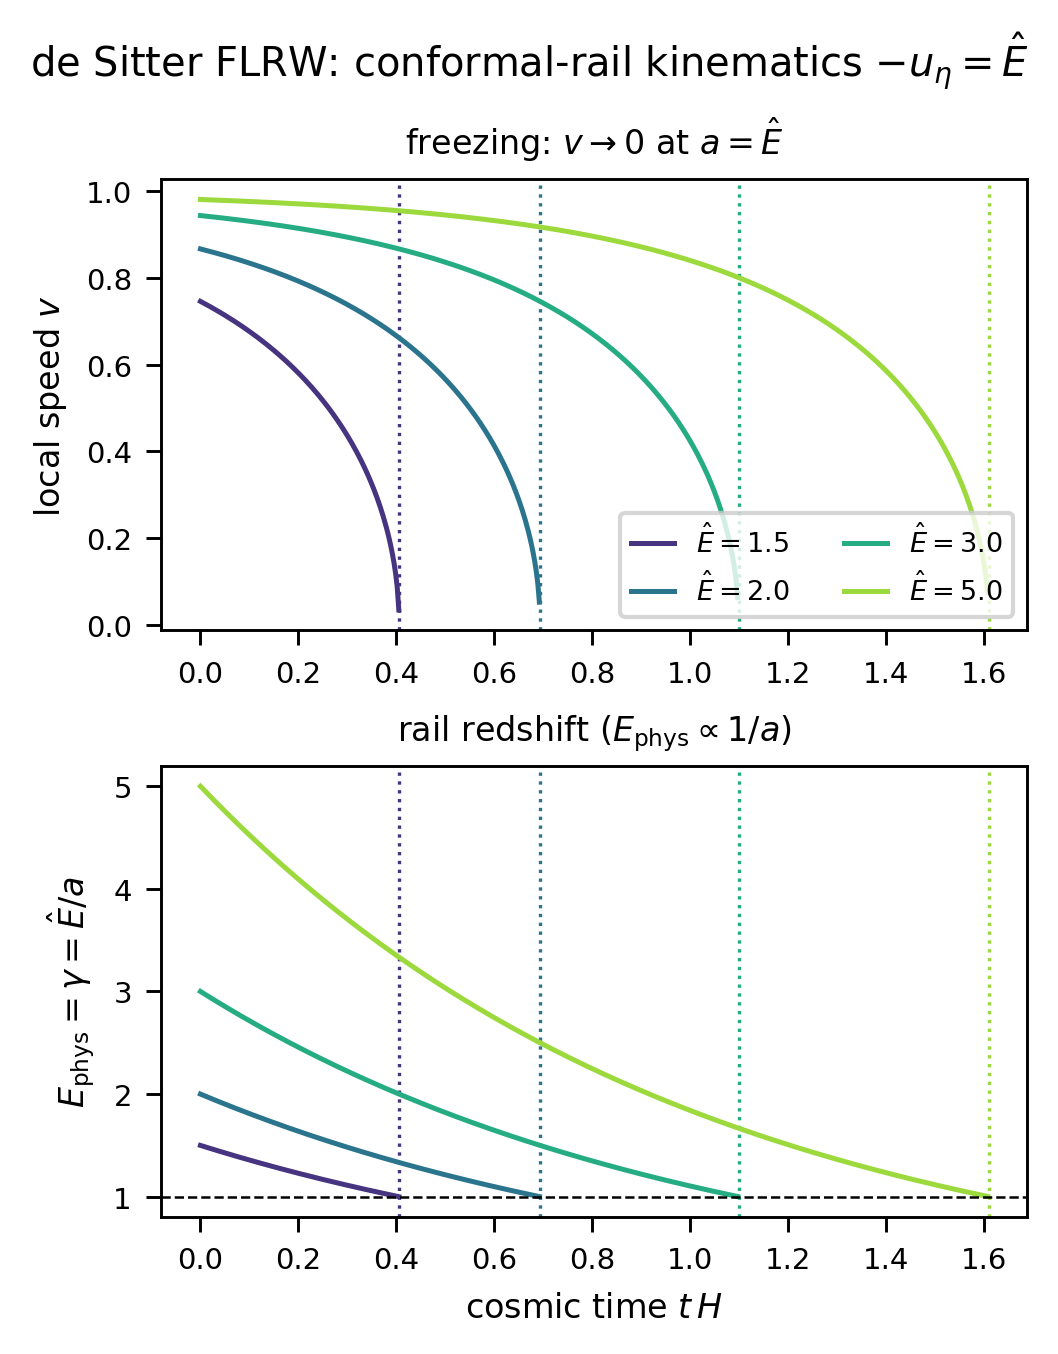
\includegraphics[width=\textwidth,height=0.68\textheight,keepaspectratio]{Immagini/fig_flrw_cinematica.png}
    \caption{de Sitter FLRW rail kinematics: local speed $v$ and rail redshift
    $E_{\rm phys}=\Ehat/a$; freezing at $a=\Ehat$.}
    \label{fig:flrw-kin}
\end{figure}


\begin{figure}[tbp]
    \centering
    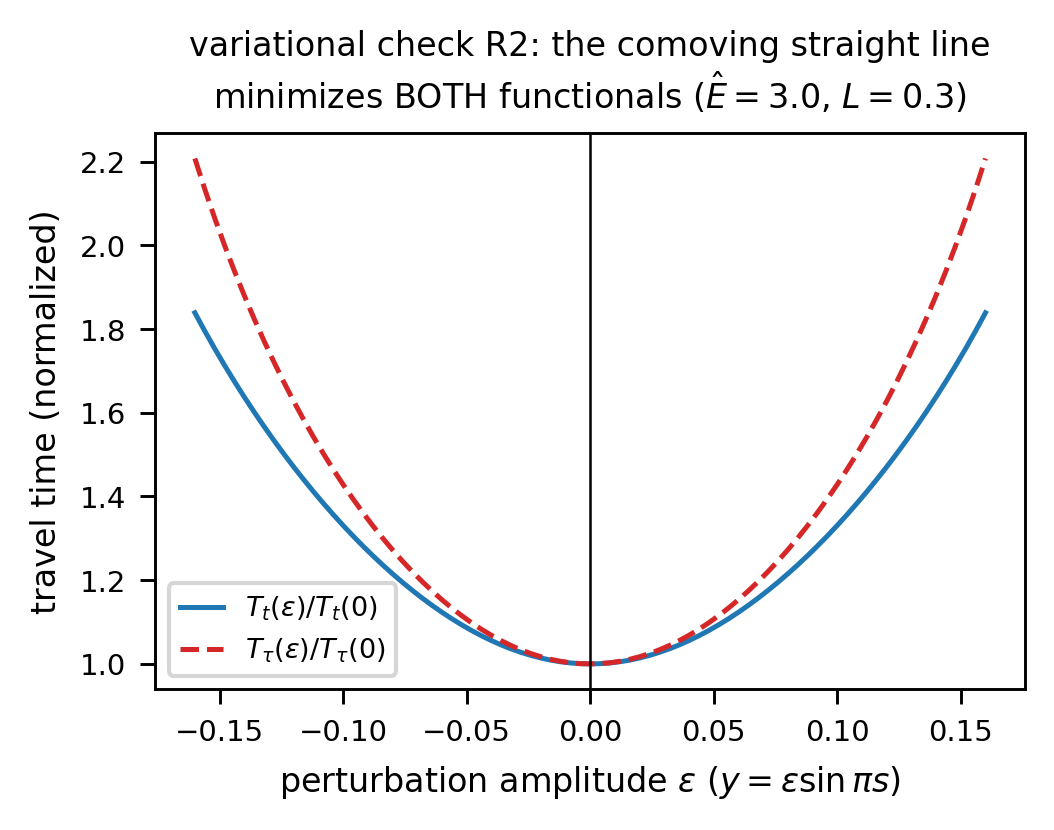
\includegraphics[width=\textwidth,height=0.68\textheight,keepaspectratio]{Immagini/fig_flrw_variazionale.png}
    \caption{Variational check: the comoving straight line minimizes
    \emph{both} $T_t$ and $T_\tau$ (branch degeneracy).}
    \label{fig:flrw-var}
\end{figure}


% ======================================================================
\section{Vaidya: dynamical black hole and the Kodama rail}
\label{sec:vaidya}
% ----------------------------------------------------------------------
The ingoing Vaidya metric $\dd s^2=-f\,\dd v^2+2\,\dd v\,\dd r+r^2\dd\Omega^2$,
$f=1-2m(v)/r$ \cite{Vaidya1951,LindquistSchwartzMisner1965}, has no timelike
Killing vector; its trapping structure is that of a dynamical horizon
\cite{AshtekarKrishnan2003,Booth2005,FaraoniBook}. The Kodama vector
\cite{Kodama1980,Hayward1996,AbreuVisser2010}
\begin{equation}
    K^a=\varepsilon^{ab}\nabla_b r = \partial_v ,\qquad
    \nabla_a K^a=0,
    \label{eq:kodama}
\end{equation}
is divergence-free without any Killing symmetry, and its charge is the
Misner--Sharp mass $m(v)$ \cite{MisnerSharp1964,HaywardMukohyama1999}.

\subsection{Kodama energy is the rail invariant}
\label{sec:kodama-energy}
From the rail constraint alone one finds the exact identity
$-g(T,T)=(f\,u^v-1)^2/\Ehat^2$, hence
\begin{equation}
    -\,u\cdot K \;=\; \Ehat \quad\text{identically along the brachistochrone.}
    \label{eq:kodama-conserved}
\end{equation}
This is \emph{controlled} conservation, not Noether: for a geodesic
$-u\cdot K$ would drift at rate $-m'(u^v)^2/r\propto m'$, exactly the
right-hand side of Eq.~\eqref{eq:cost} for $W=K$. Only the unnormalized
$K=\partial_v$ has zero control cost in the static limit; the normalized
$\hat K=K/\sqrt f$ does not (discriminating test), which is why the Kodama
vector, not a unit selector, is the canonical choice.

\paragraph{Indicatrix and Hamiltonians.} With $w\equiv\Ehat^2-f$ the constraint
$-u_v=\Ehat$ turns the admissible velocities at fixed $(v,r)$ into an ellipse,
\begin{equation}
    r'=(f-\Ehat^2)+\Ehat\sqrt w\,\cos\theta,\qquad
    \varphi'=\frac{\sqrt w}{r}\sin\theta,
    \label{eq:vaidya-ind}
\end{equation}
a Zermelo problem with ingoing radial wind $f-\Ehat^2<0$. Maximizing
$p\cdot\dot x$ over $\theta$ at fixed $p_\varphi=J$ gives the closed-form branch
Hamiltonians
\begin{align}
    H_v&=p_r(f-\Ehat^2)-1+\sqrt w\,\sqrt{\Ehat^2 p_r^2+J^2/r^2},
    \label{eq:Hv}\\
    H_\tau&=p_r(f-\Ehat^2)-\Ehat
        +\sqrt w\,\sqrt{(\Ehat p_r+1)^2+J^2/r^2}.
    \label{eq:Htau-vaidya}
\end{align}
The $\tau$-branch is the $v$-branch under $p_r\to p_r+1/\Ehat$ with unit cost
replaced by $\Ehat$. Non-stationarity is the explicit dependence
$\dd H/\dd v=\partial_v H\propto m'(v)$; the teleological momentum $p_v=-H$
satisfies $p_v(r_1)=0$ at the free arrival radius yet $p_v(r)\neq0$ along the
path, so the turning point \emph{anticipates future accretion}
(Fig.~\ref{fig:vaidya-traj}).

\begin{figure}[ht]
    \centering
    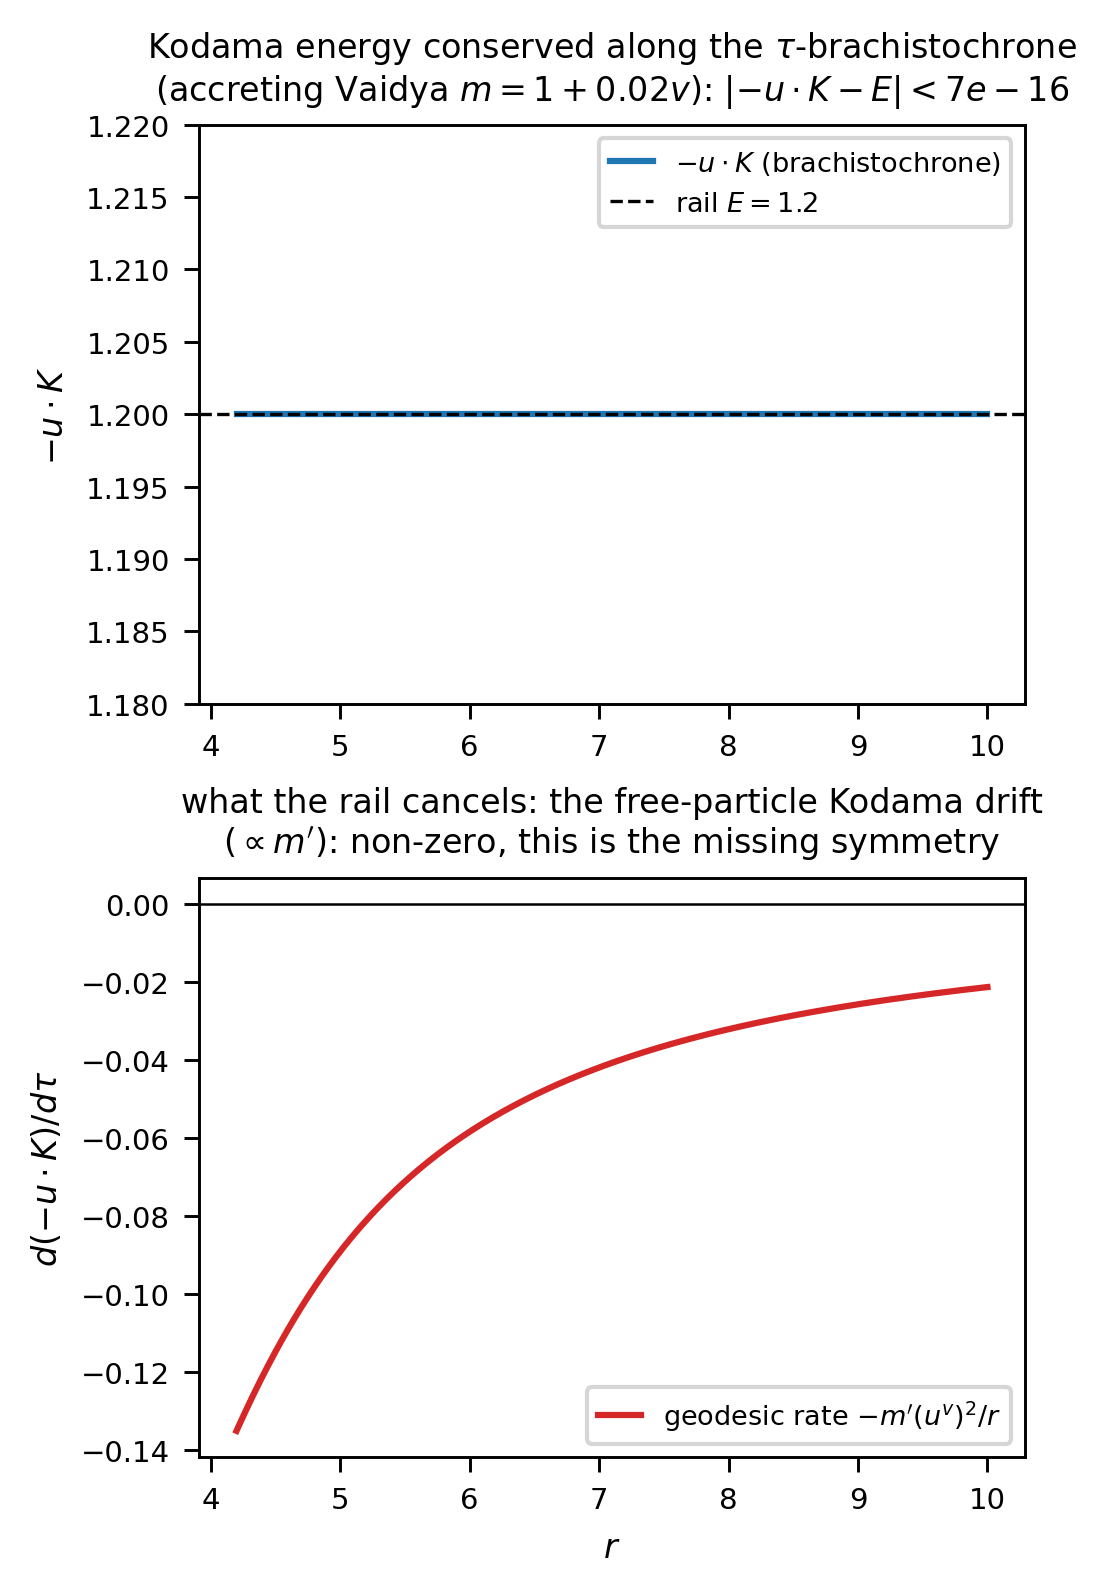
\includegraphics[width=\textwidth,height=0.68\textheight,keepaspectratio]{Immagini/fig_kodama_conservazione.png}
    \caption{Kodama energy $-u\cdot K=\Ehat$ conserved along the
    $\tau$-brachistochrone to $6.7\times10^{-16}$ (top); the free-particle
    drift $\propto m'$ that the rail cancels (bottom).}
    \label{fig:kodama}
\end{figure}


\subsection{Phenomenology: penetration, timing, bounce}
\label{sec:vaidya-pheno}
Three features distinguish the dynamical hole from its frozen-mass
Schwarzschild limit.

\emph{Penetration.} The $\tau$-brachistochrone reaches the apparent horizon
$r=2m(v)$ only if $|J|$ lies below a threshold $J_c(v_0)$; accretion ($m'>0$)
opens a \emph{finite} window $J_c>0$, whereas evaporation ($m'<0$) closes it to
zero measure---an accretion/evaporation asymmetry with no static analogue. The
finite capture interval $J\in(0,\Jc]$ is the analogue of the Kerr $t$-branch
dichotomy, generated here by the \emph{dynamics}: grazing orbits linger near
periapsis while the growing horizon closes the gap.

\emph{Bounce.} The $r$-parametrization degenerates at periapsis
($\dd v/\dd r\to\infty$); reparametrizing by $v$ makes the Euler--Lagrange
problem regular at the turning point $r'=0$, so the trajectory is integrated
straight \emph{through} the bounce---the same extremal, via the exact change of
variable $(f v'-1)\dd r=(f-r')\dd v$. The $v$-flow reaches the periapsis exactly
where the $r$-flow diverges ($r_{\min}=3.0105$ at $v=7.29$ for $\mu\equiv m'=0.01$),
and the teleological memory $p_v(r)\propto m'$ measures the departure from the
frozen-mass Schwarzschild curve (Fig.~\ref{fig:vaidya-bounce}).

\emph{Timing and the orbit--horizon race.} Because $m$ grows along the path,
$r_{\min}$ depends on \emph{when} the particle arrives, the epoch $v_1$---a
genuinely non-stationary effect absent in Kerr. Strikingly, the absolute and
relative penetration have \emph{opposite} winners
(Fig.~\ref{fig:vaidya-timing}): under evaporation the absolute periapsis descends
but the horizon $2m(v)$ retreats faster, so the relative penetration
$r_{\min}/2m(v_{\rm peri})$ \emph{worsens} for later arrivals; under accretion the
periapsis rises yet the horizon grows faster, so late arrivals graze the relative
horizon. The orbit--horizon chase has reversed outcomes measured in $r$ versus in
horizon units.

\begin{figure}[ht]
    \centering
    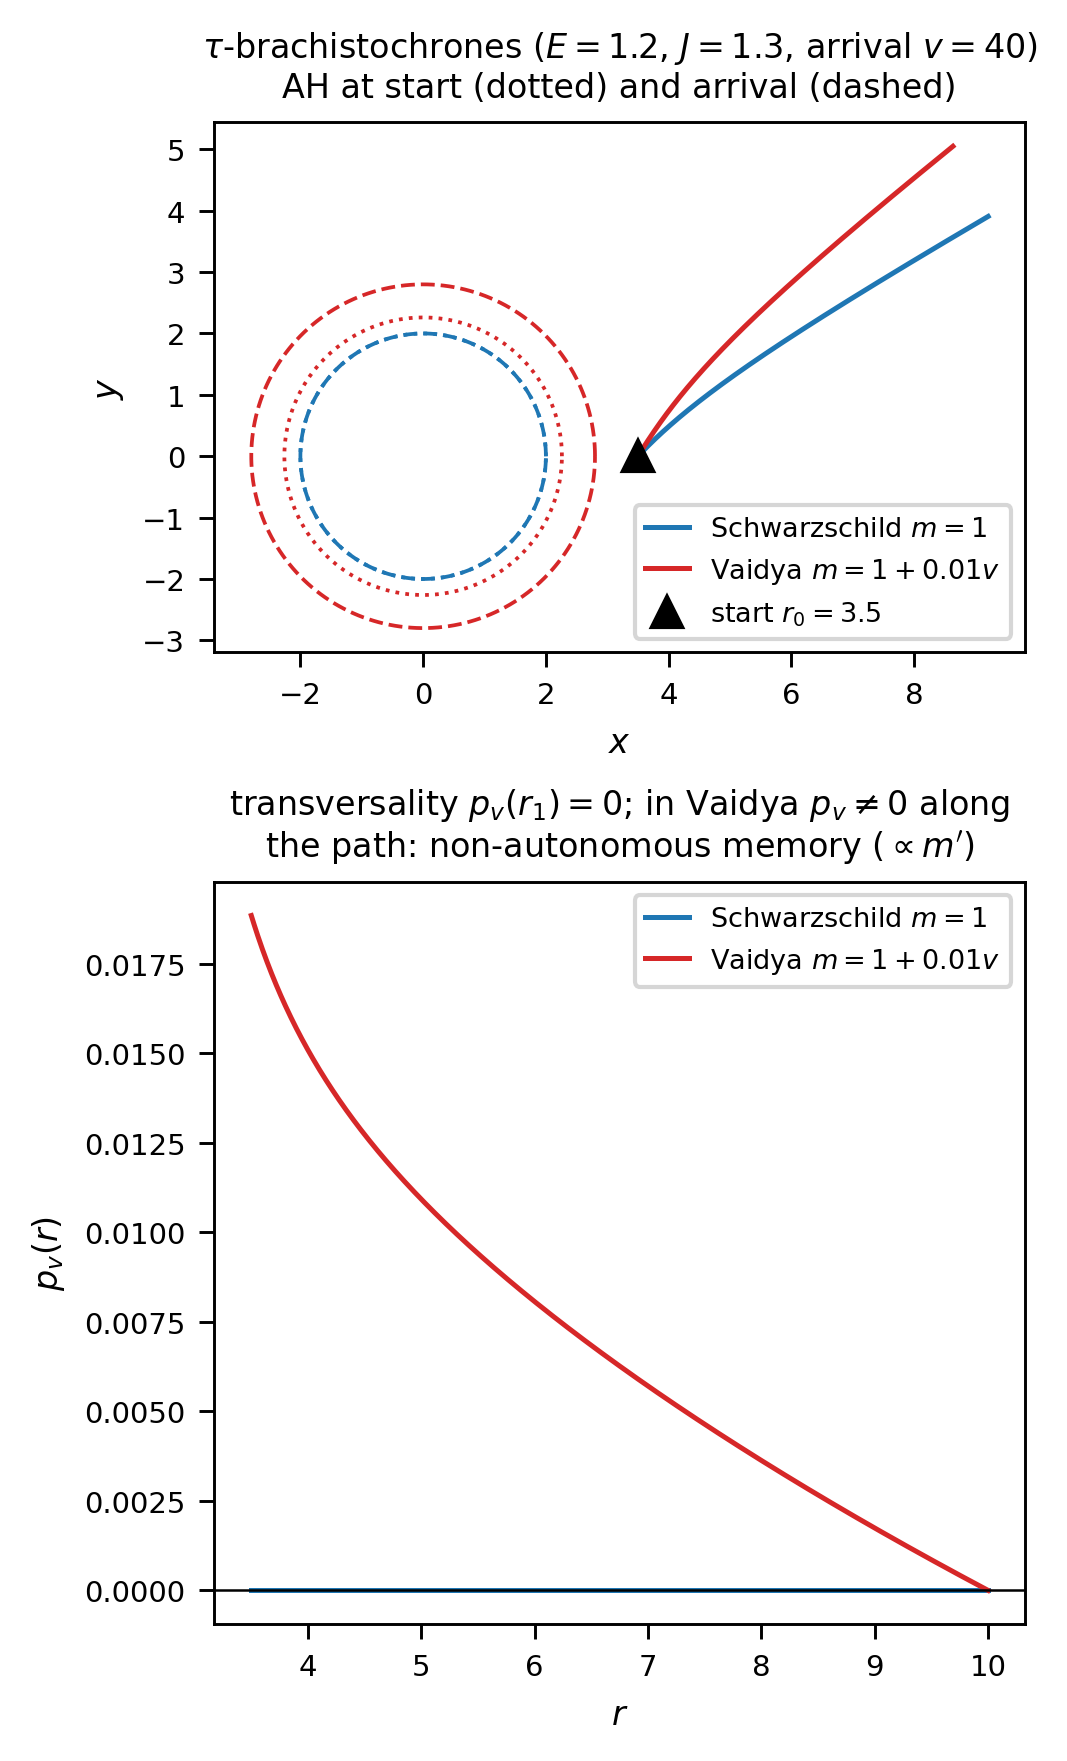
\includegraphics[width=\textwidth,height=0.68\textheight,keepaspectratio]{Immagini/fig_vaidya_traiettorie.png}
    \caption{$\tau$-brachistochrones Schwarzschild vs Vaidya, and $p_v(r)$:
    transversality $p_v(r_1)=0$, non-autonomous memory $\propto m'$.}
    \label{fig:vaidya-traj}
\end{figure}


\subsection{Plunge-radius law and the (absent) evaporative inversion}
\label{sec:vaidya-plunge}
The turning-point law has the static Schwarzschild form evaluated at the mass
at periapsis, $f_*=1-2m(v_{\rm peri})/r_{\min}$:
\begin{align}
    \tau:&\quad (\Ehat^2-f_*)J^2 = f_* r_{\min}^2 ,\\
    t:&\quad (\Ehat^2-f_*)J^2 = \Ehat^2 r_{\min}^2/f_* ,
    \label{eq:vaidya-turn}
\end{align}
plus a genuine $O(m')$ correction from the teleological momentum $p_v$. The
static ratio $J^2_t/J^2_\tau=\Ehat^2/f^2>1$ gives $r_{\min}^t<r_{\min}^\tau$
(``$t$ deeper''), robust for physical evaporation: \emph{there is no physical
evaporative inversion} (the apparent linear-model inversion is an artifact of
$m\le0$).

\begin{figure}[ht]
    \centering
    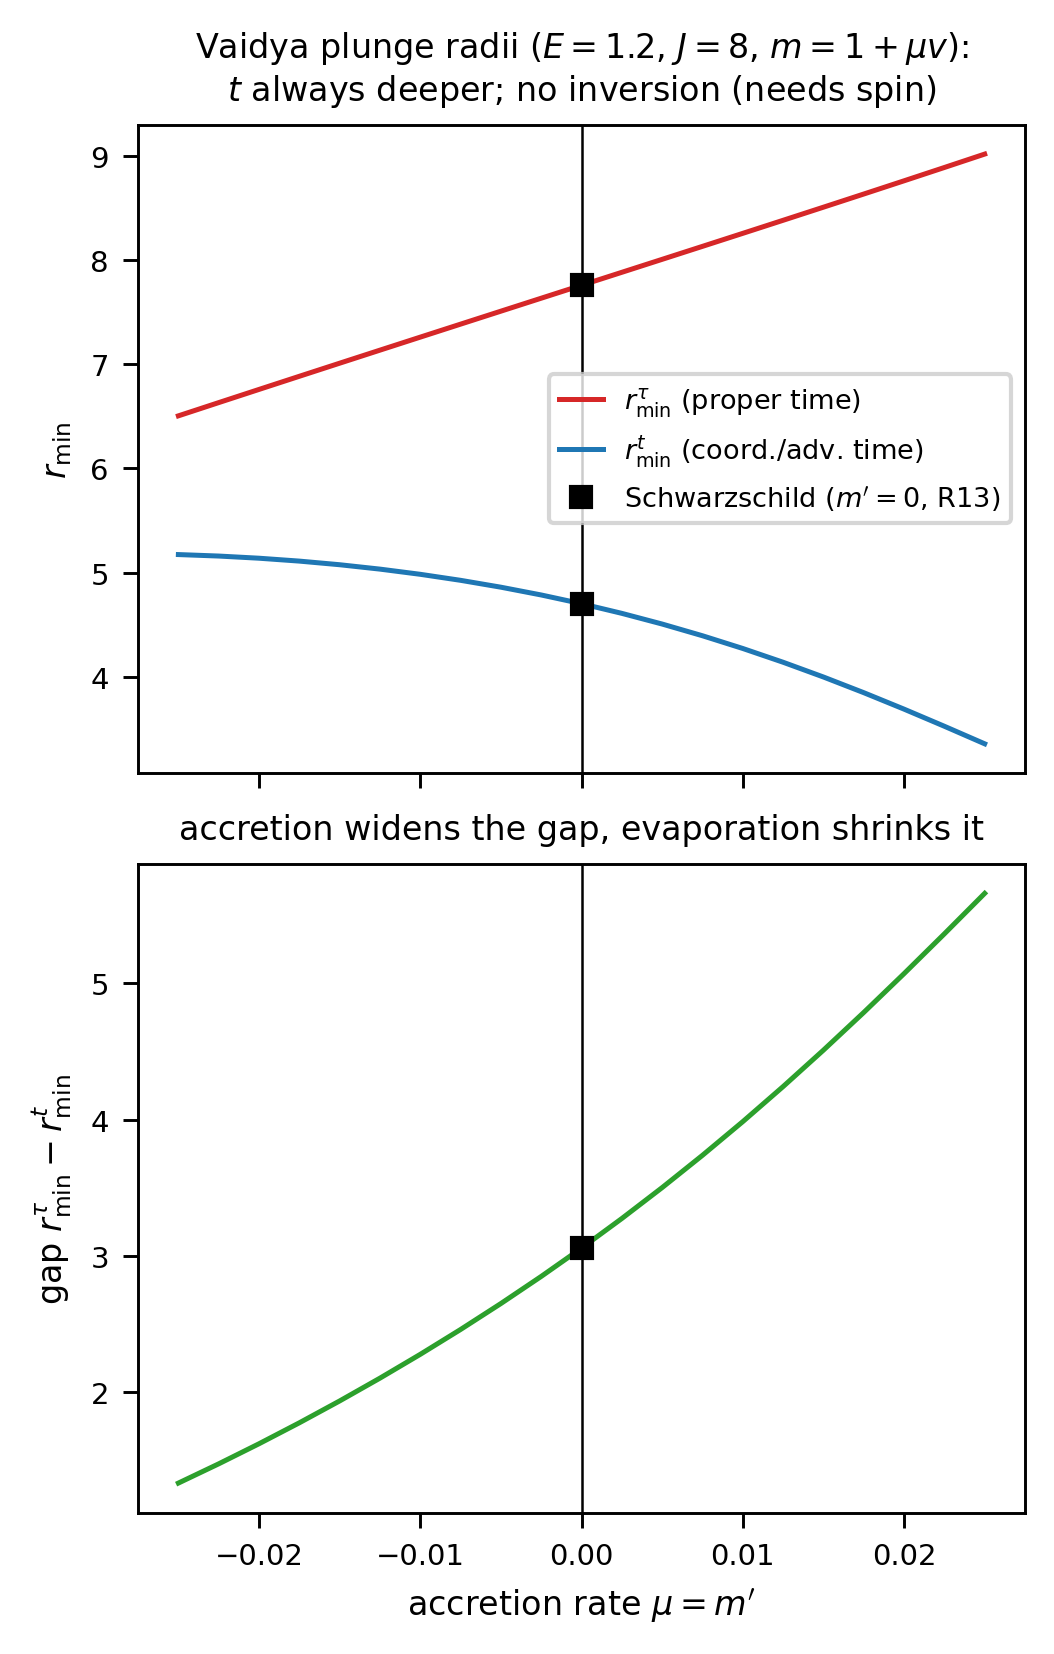
\includegraphics[width=\textwidth,height=0.68\textheight,keepaspectratio]{Immagini/fig_vaidya_plunge_t_tau.png}
    \caption{Plunge radii $r_{\min}^{t,\tau}$ and gap vs $\mu=m'$; $t$ deeper,
    accretion widens the gap.}
    \label{fig:vaidya-plunge}
\end{figure}

\begin{figure}[ht]
    \centering
    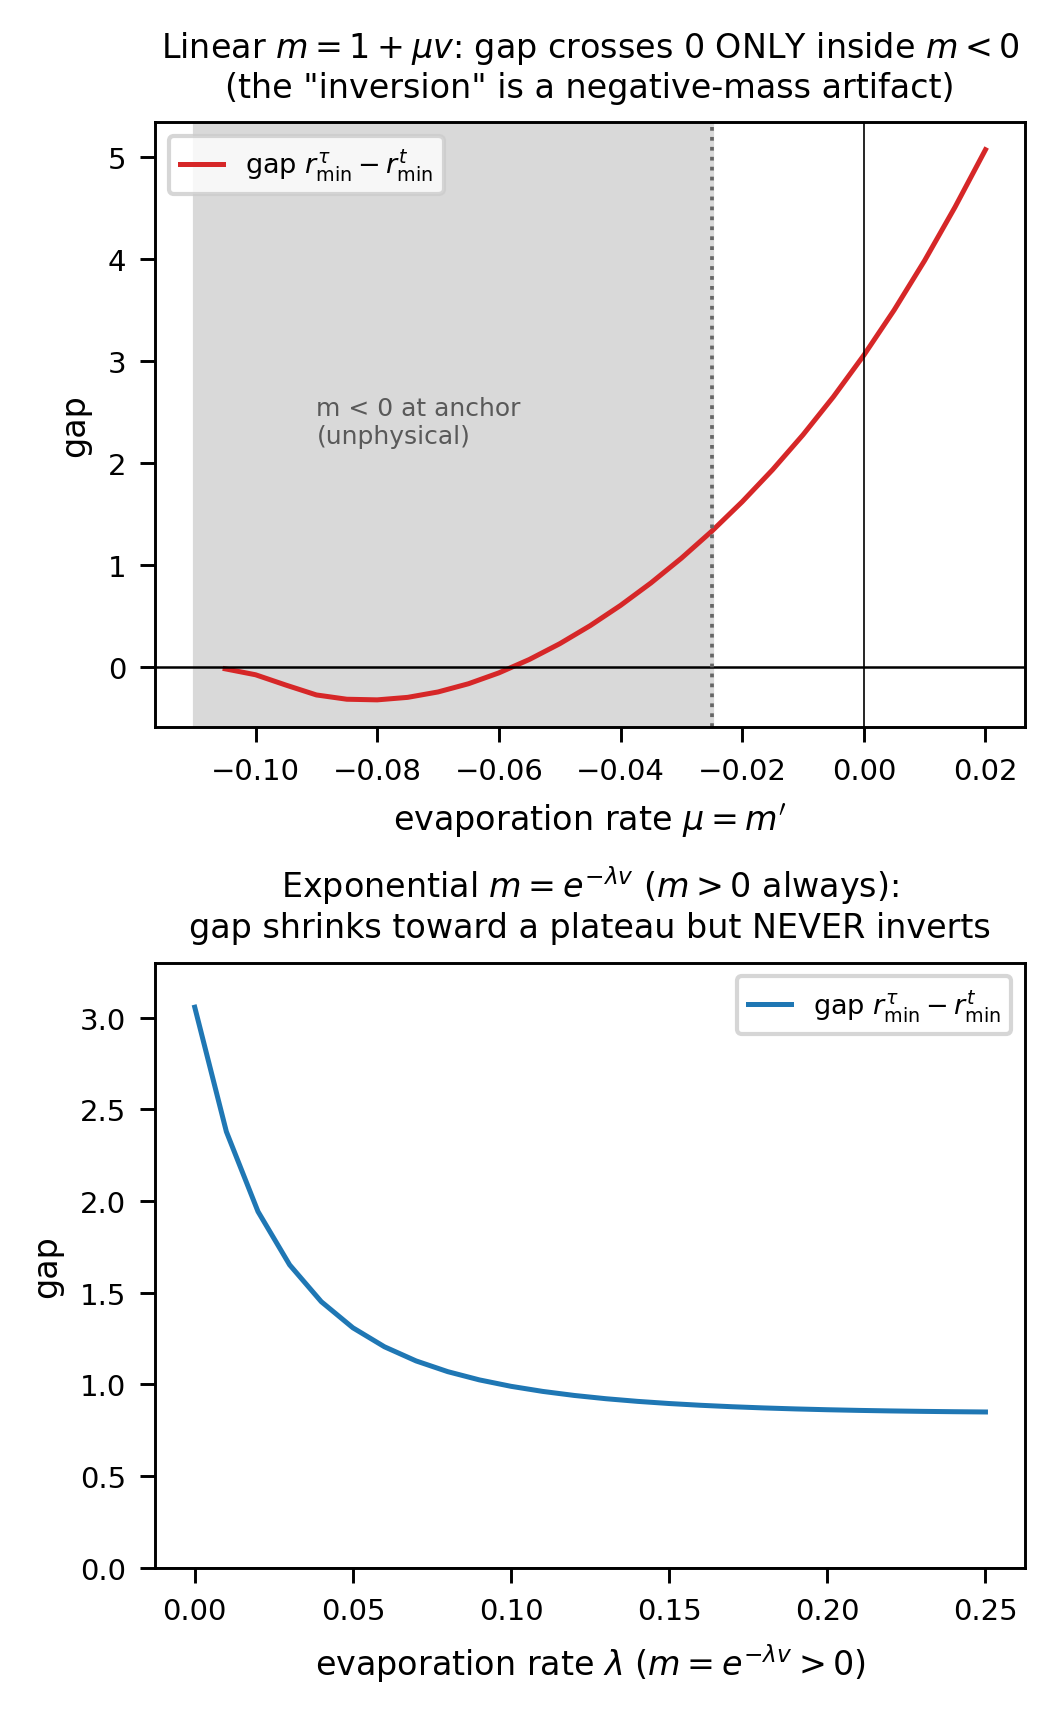
\includegraphics[width=\textwidth,height=0.68\textheight,keepaspectratio]{Immagini/fig_vaidya_no_inversione_evaporazione.png}
    \caption{No physical evaporative inversion: the linear-model sign change
    lies entirely in the unphysical $m<0$ region; with $m=e^{-\lambda v}>0$ the
    gap shrinks but never inverts.}
    \label{fig:vaidya-noinv}
\end{figure}


% ======================================================================
\section{Thakurta--Kerr: conformal rotating compact object}
\label{sec:thakurta}
% ----------------------------------------------------------------------
Thakurta--Kerr is conformal Kerr, $g=A(\eta)^2 g_{\rm Kerr}$
\cite{Thakurta1981,Kerr1963}, one of a family of cosmological geometries
\cite{McVittie1933,SultanaDyer2005,Kaloper2010,NolanMcVittie1998,MelloMaciel2017,FaraoniBook}.
For constant $A$
the transfer theorem maps the problem to Kerr with $E_{\rm eff}=\Ehat/A$,
$J_{\rm eff}=J/A$; the horizon $\rp$ is rigid (conformally invariant), the
ergosphere $\re=2M$ is crossed regularly, while the freezing surface
$A^2 f=\Ehat^2$ breathes.

\paragraph{Indicatrix and Hamiltonians.} Equatorially, write
$\Delta=r^2-2Mr+s^2$, $\bar v^2=1-A^2f/\Ehat^2$, and
$\bar P=P+A^2(2Ms/r)^2/\Ehat^2$ with $P=r^2+s^2+2Ms^2/r$. The rail
$\Ehat=-u_\eta$ makes the indicatrix an ellipse with an \emph{azimuthal} wind
(frame dragging),
\begin{equation}
    \varphi'_0=\frac{2Ms}{r}\frac{\bar v^2}{\bar P},\qquad
    R^2=f\bar v^2+\bar P\varphi_0'^2=\frac{\Delta\,\bar v^2}{\bar P},
    \label{eq:tk-ind}
\end{equation}
the last equality using the Kerr identity $fP+(2Ms/r)^2=\Delta$. The
conformal-time, coordinate-time and proper-time Hamiltonians are
\begin{align}
    H_\eta&=p_\varphi\varphi'_0
        +R\sqrt{(\Delta/r^2)p_r^2+p_\varphi^2/\bar P}-1,
    \label{eq:Heta}\\
    H_t&=p_\varphi\varphi'_0
        +R\sqrt{(\Delta/r^2)p_r^2+p_\varphi^2/\bar P}-A,
    \label{eq:Ht-tk}\\
    H_\tau&=\tilde p_\varphi\varphi'_0
        +R\sqrt{(\Delta/r^2)p_r^2+\tilde p_\varphi^2/\bar P}-\frac{A^2 f}{\Ehat},
    \label{eq:Htau-tk}
\end{align}
with the conformal gravitomagnetic shift
$\tilde p_\varphi=p_\varphi-2MsA^2/(r\Ehat)$. The arrival-time branch $H_t$ differs
from $H_\eta$ only in the unit cost ($-1\to-A$) and reduces to it for $A=1$; it is
the branch compared with $\tau$ in the plunge inversion
(Sec.~\ref{sec:inversion}), where its turning potential
$H_{t0}=H_t|_{p_r=0}$ enters. All three are regular through the
ergosphere ($f=0\Rightarrow R^2=\bar v^2\Delta/\bar P>0$) and degenerate only at
the horizon $\Delta=0$, which is therefore conformally invariant---independent of
$A$ and $\Ehat$. The three branches share this ellipse: $t$ follows the same
curves as $\eta$ through $t=\int A\,\dd\eta$, while $\tau$ is Riemannian-pure, the
wind cancelling the gravitomagnetic term, so it survives the expansion
(Fig.~\ref{fig:th-branches}).

\paragraph{Non-autonomous optical reduction.} Solving the indicatrix for
$\dd\eta$ at fixed spatial displacement casts the $\eta$-branch as a closed-form
Randers metric, non-autonomous through the conformal factor,
\begin{align}
    \dd\eta &= n(\eta,r)\,\alpha_K+\beta_K,\qquad
    n=\frac{\Ehat}{\sqrt{\Ehat^2-A^2 f}},
    \label{eq:randers}\\
    \alpha_K^2 &= \frac{r^2\,\dd r^2}{f\Delta}+\frac{\Delta\,\dd\varphi^2}{f^2},
    \qquad
    \beta_K = -\frac{2Ms}{rf}\,\dd\varphi.
    \label{eq:randers-data}
\end{align}
The Riemannian data $\alpha_K$ and the one-form $\beta_K$ are \emph{exactly} those
of the \emph{null} Fermat (Randers) metric of Kerr \cite{GibbonsWerner2008}: all
of the mass, rail, and expansion physics is carried by the scalar index $n$,
which multiplies only the Riemannian part, while the frame-dragging one-form
$\beta_K$ is rigid---conformally invariant and independent of $\Ehat$. The
reduction is thus a Zermelo problem with a time-dependent landscape in which only
the metric term breathes, not the wind. It degenerates at the ergosphere ($f=0$,
where $1/F$ is intrinsic, as for stationary Kerr) even though the
Hamiltonian~\eqref{eq:Heta} remains regular there; the limits $\Ehat\to\infty$
(null Kerr optics), $A=1$ (stationary Perlick on Kerr), $s=0$
(Thakurta--Schwarzschild) and $M=s=0$ ($n=1/v$, FLRW) are all recovered.



\begin{figure}[ht]
    \centering
    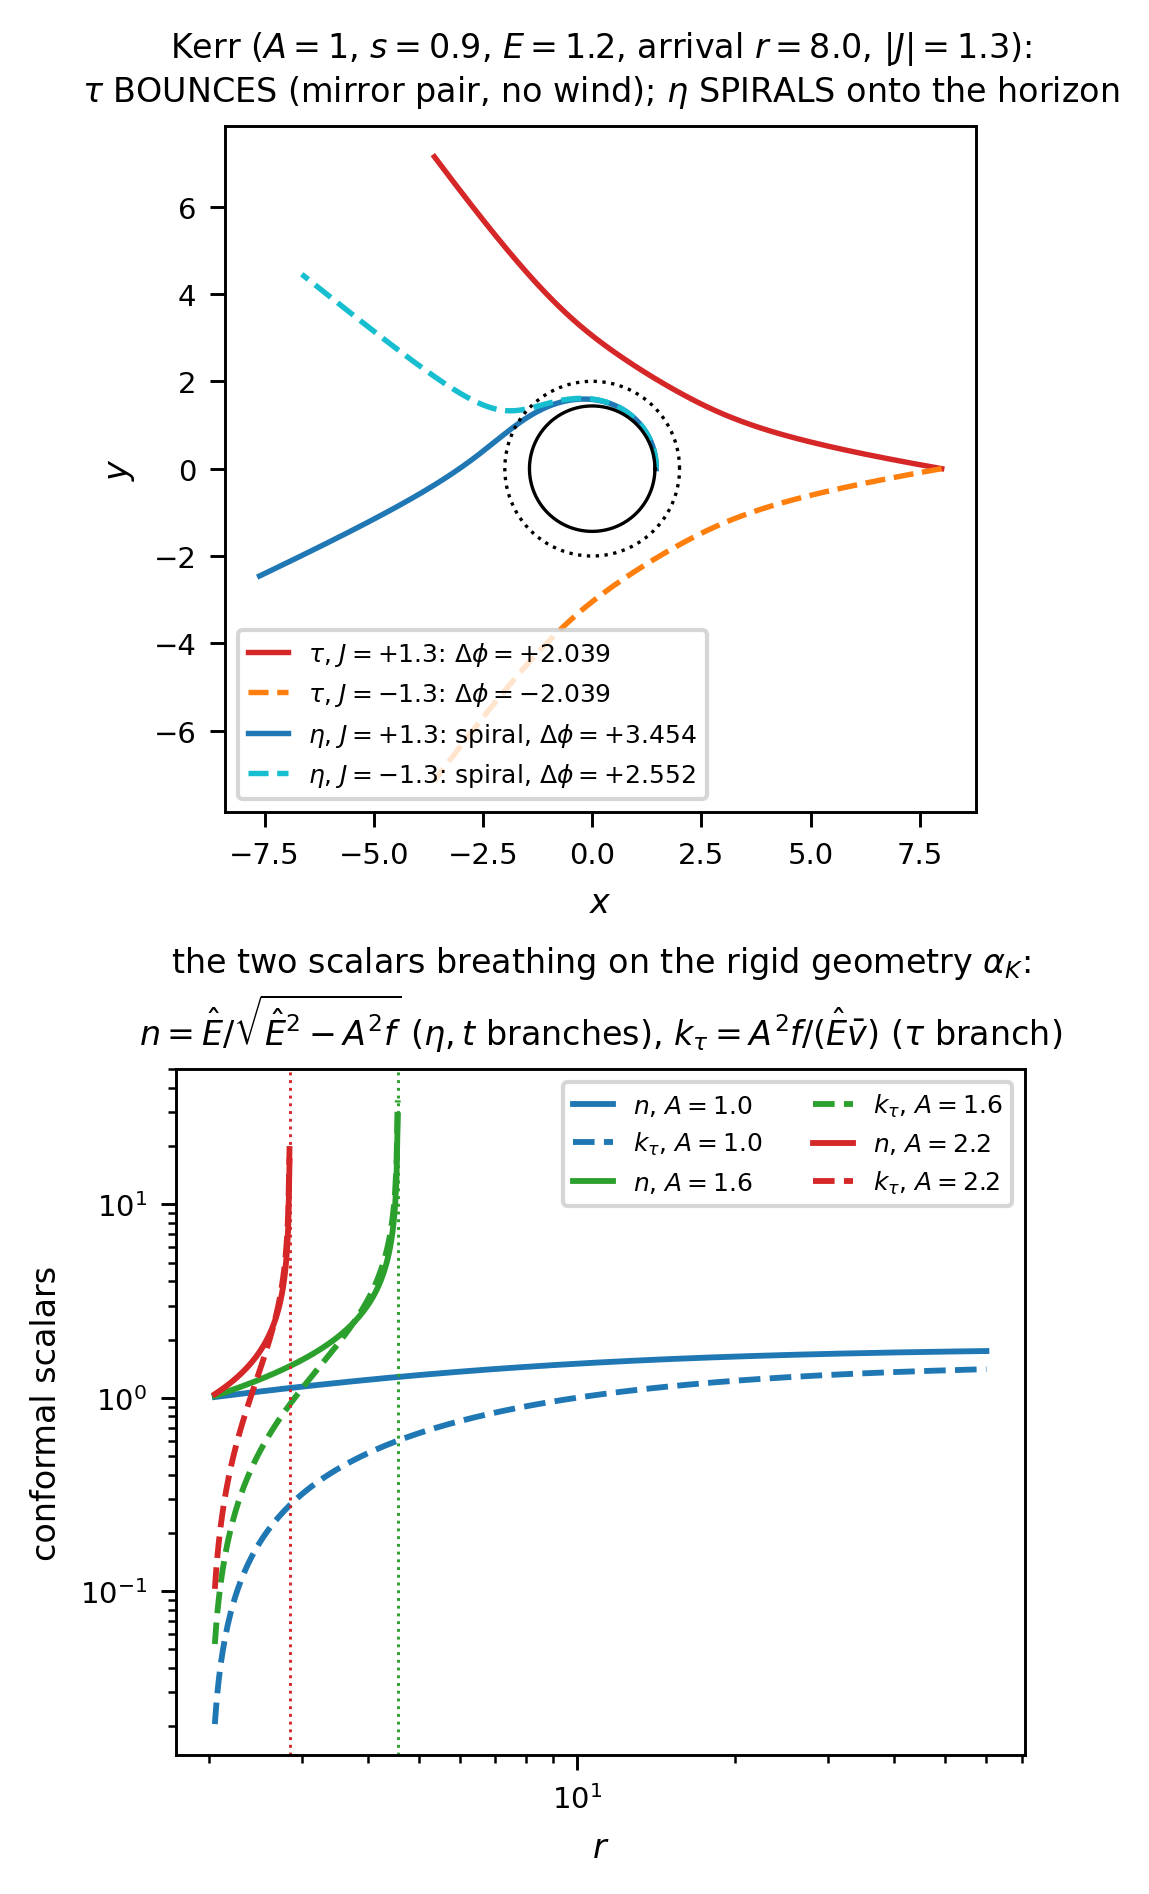
\includegraphics[width=\textwidth,height=0.68\textheight,keepaspectratio]{Immagini/fig_thakurta_kerr_rami.png}
    \caption{The three branches: $\tau$ bounces (mirror pair, no wind), $\eta$
    spirals (gravitomagnetic wind); breathing conformal scalars $n,k_\tau$.}
    \label{fig:th-branches}
\end{figure}

\subsection{Quasi-constants and drift}
\label{sec:quasiconst}
For constant $A$ the transfer theorem is exact at the level of conserved
quantities: $u_{\rm TK}=u_{\rm K}/A$ maps the $\Ehat$-rail onto the Kerr rail with
$E_{\rm eff}=\Ehat/A$, so every Kerr quasi-constant carries over by substitution,
\begin{equation}
    K^{\rm TK}=K^{\rm Kerr}(E_{\rm eff}),\qquad
    K_\tau=Q_{\rm std}+a^2 f_2\,p_\theta^2+O(a^4),
    \label{eq:Ktransfer}
\end{equation}
with $Q_{\rm std}$ the Carter constant and $f_2$ the next-to-leading polar
coefficient \cite{Carter1968,RosignoliKerr}. The polar libration that carries the
quasi-constant lives off the equatorial plane, governed by the full Hamiltonian
on a generic slice $\Sigma=r^2+s^2\cos^2\theta$,
\begin{equation}
    H_\tau=\tilde p_\varphi\varphi'_0
      +R\sqrt{\frac{\Delta}{\Sigma}p_r^2+\frac{p_\theta^2}{\Sigma}
      +\frac{\tilde p_\varphi^2}{\bar G}}-\frac{A^2 f_\Sigma}{\Ehat},
    \label{eq:H3d}
\end{equation}
with $f_\Sigma=1-2Mr/\Sigma$, $b=2Mar\sin^2\theta/\Sigma$,
$\bar G=G+A^2 b^2/\Ehat^2$, $\tilde p_\varphi=J-A^2 b/\Ehat$,
$\varphi'_0=b\bar v_\Sigma^2/\bar G$, $R^2=\bar v_\Sigma^2\Delta\sin^2\theta/\bar G$,
and the block identity $f_\Sigma G+b^2=\Delta\sin^2\theta$; it reduces to
Eqs.~\eqref{eq:Heta}--\eqref{eq:Htau-tk} on the equator. For $A=A(\eta)$ the
substitution~\eqref{eq:Ktransfer} is only the zeroth order: the transport equation
$\dd K/\dd\lambda=\{K,H\}+\partial_\eta K$ acquires an explicit source at order
$a^2\varepsilon$, $\varepsilon=A'/A$,
\begin{equation}
    \frac{\dd K}{\dd\eta}\bigg|_{\rm expl}=\varepsilon\,a^2\,S_1,\qquad
    S_1=2E_{\rm eff}^2\!\left[\cos^2\theta
        +\frac{M\cos2\theta\,p_\theta^2}{r\,DE_0^2}\right],
    \label{eq:S1}
\end{equation}
where $DE_0=r^2 w_{\rm eff}$. The counterterm $h$ solving $\{h,H_0\}=-S_1$
inherits the double pole at the \emph{freezing wall}
$r_w=2M/(1-E_{\rm eff}^2)$, so the dynamical quasi-constant is
\begin{equation}
    K^{\rm TK}(\eta)=K^{\rm Kerr}\!\big(E_{\rm eff}(\eta)\big)
        -a^2\!\int\!\varepsilon\,S_1\,\dd\eta,
    \label{eq:Kdyn}
\end{equation}
with closed toroidal averages
$\langle S_1\rangle=E_{\rm eff}^2(1-J^2/L^2)
+2ME_{\rm eff}^2|J|(L-|J|)/(r\,DE_0^2)$, $L^2=p_\theta^2+J^2/\sin^2\theta$. In
Kerr ($E>1$) the wall is absent; in Thakurta--Kerr with $E_{\rm eff}<1$ it enters
from the far field and advances inward as $A$ grows, becoming a \emph{global
attractor}: the bound $\tau$-libration ceases to exist, so the dynamical
quasi-constants live on scattering arcs ($E_{\rm eff}>1$) or on the $t$-branch.




% ======================================================================
\section{Equatorial closed forms and the ergosphere}
\label{sec:closed}
% ----------------------------------------------------------------------

\subsection{Separatrix in Weierstrass functions}
\label{sec:separatrix}
From the doranTau factorization $\Delta-\Jc^2 w=f(r^2+c^2)$, $c=a/E$
\cite{RosignoliKerr}, the
equatorial $\tau$-separatrix $\varphi(r)$ is genus~1, closed in the
Weierstrass functions $\wp,\sigma,\zeta$
\cite{WhittakerWatson,DLMF,Hackmann2008,Hackmann2010}: the angle is linear in the
uniformizing variable $z(r)=\wp^{-1}(A/r+B)$ plus two $\sigma$-ratios
[App.~\ref{app:explicit}, Eq.~\eqref{eq:sep-phi}], regular \emph{through} the
ergosphere because the factor $r^2+c^2$ divides the turning quartic and removes
$\re$ from the radicand. The Boyer--Lindquist form winds logarithmically at the
horizon; the Doran shift---a second, quasi-lemniscatic elliptic
curve---cancels it, so the ergosphere-penetrating separatrix
$\varphi_D=\varphi_{\rm BL}+\varphi_{\rm shift}$ is closed on two elliptic curves.

What controls the reduction is the \emph{genus} of the turning radical, not the
rationality of $\mathcal K$. Being Riemannian-pure
(Sec.~\ref{sec:thakurta}, the gravitomagnetic wind cancels), the $\tau$-branch
factorizes as doranTau---the factor $r^2+c^2$ dividing the quartic---dropping a
generically genus-2 reduction to genus~1. Generic $t$-branch orbits carry the
wind and have the sextic radical
$\mathcal R(r)=r\,Q_2(r)\,[(E^2-1)r+2M]$ (genus~2, hyperelliptic), with no such
cancellation. The $t$-brachistochrone nonetheless has its own genus-1 closed-form
separatrix, by a \emph{different} mechanism: at the marginal-capture (saddle-node)
momentum $J_c^-$ [Eq.~\eqref{eq:Jc-minus}] the sextic develops a \emph{double
root}, $\mathcal R=(r-r_*)^2 Q_4$ with $Q_4$ quartic (whereas the prograde
ergosphere crossing $J_+^t$ has only a simple root and stays genus~2). The double
root drops the radical to $Q_4$, and $\varphi(r)$ closes in the same
Weierstrass $\wp,\sigma,\zeta$ form as the $\tau$-separatrix
(App.~\ref{app:explicit}). Both separatrices are thus genus~1---the $\tau$ one
via the doranTau factorization, the $t$ one via a double root---while generic
(non-separatrix) $t$-orbits are genuinely genus~2, closed only in genus-2
Kleinian functions.
The Kerr geodesic structure and its constants are classical
\cite{Carter1968,Chandrasekhar}. Validated end-to-end to
$2.8\times10^{-10}$ through the ergosphere, and general across parameters.

\begin{figure}[ht]
    \centering
    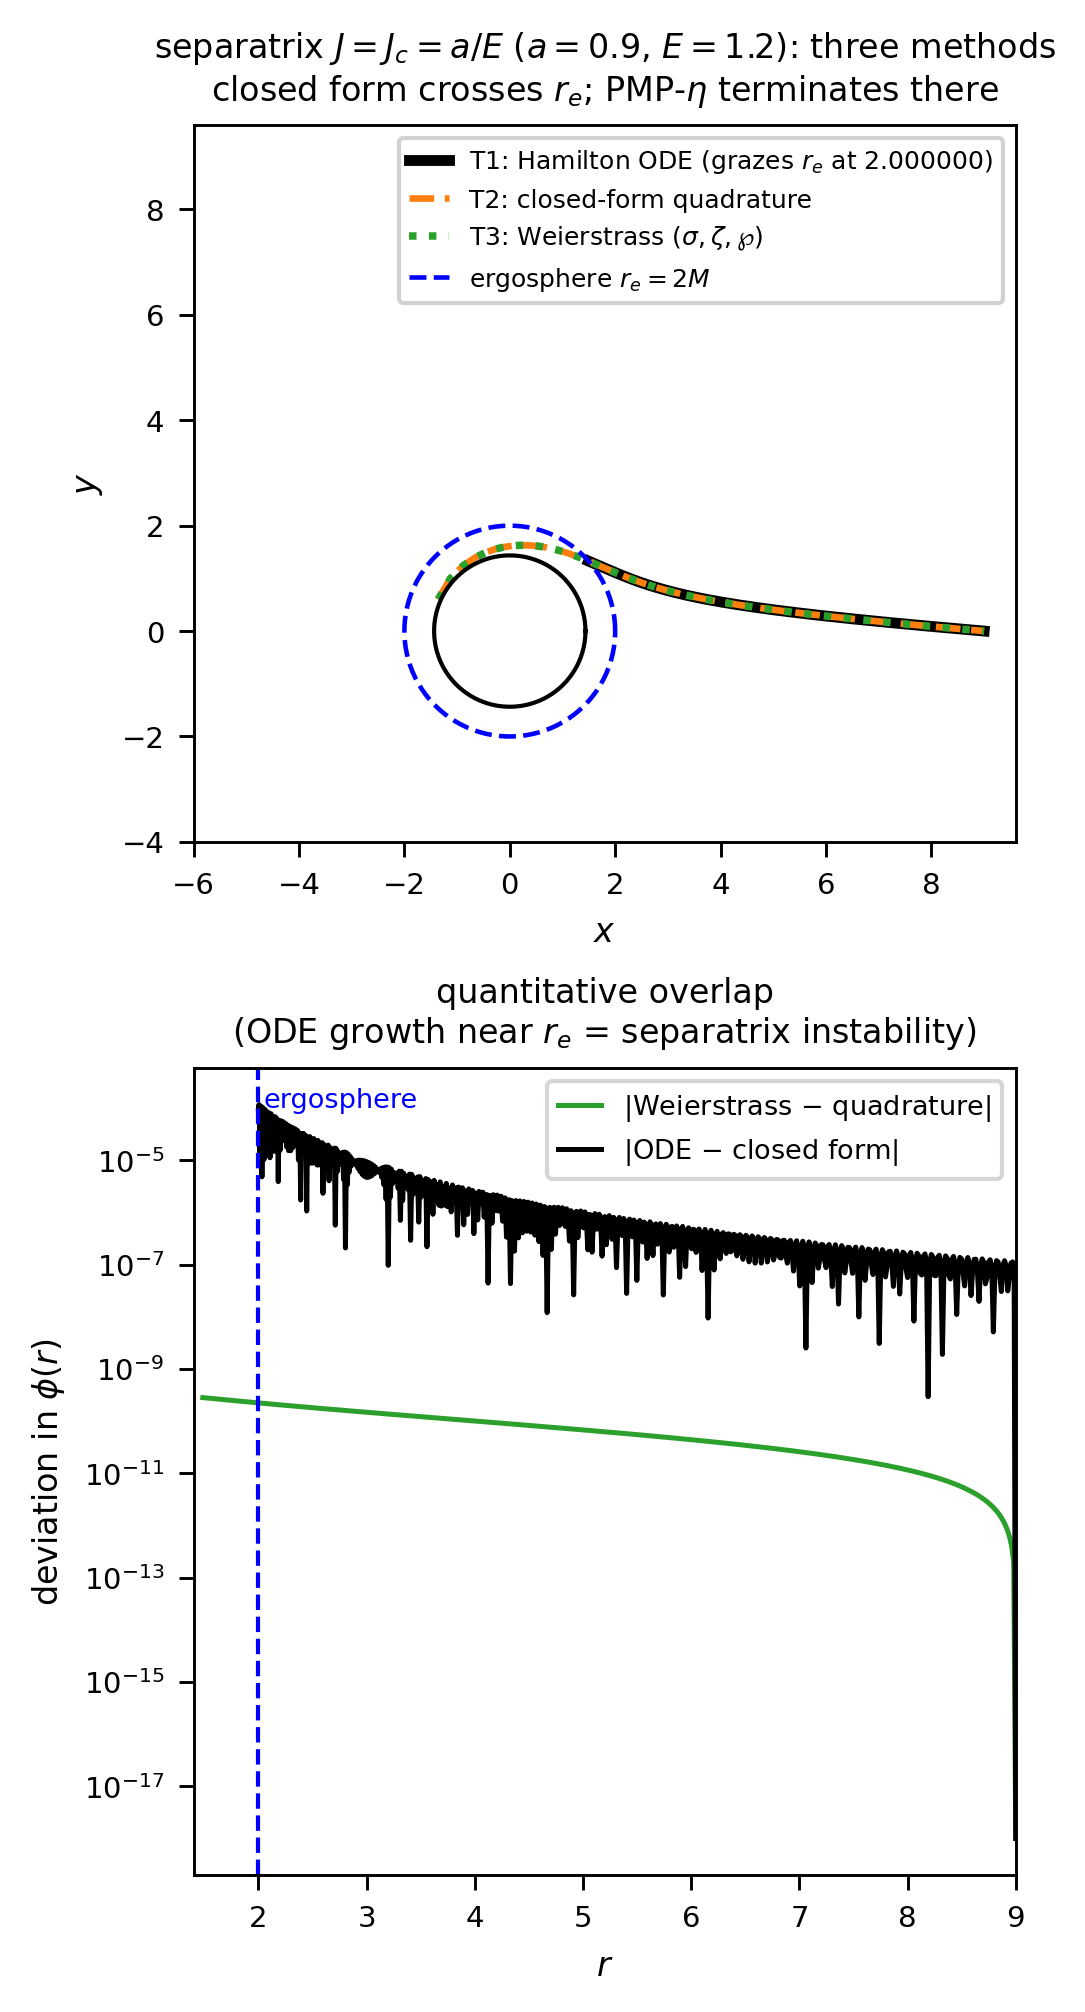
\includegraphics[width=\textwidth,height=0.68\textheight,keepaspectratio]{Immagini/fig_separatrix_3traiettorie.png}
    \caption{$\tau$-branch separatrix $J=\Jc$: ODE, quadrature and evaluated
    Weierstrass agree to $2.8\times10^{-10}$; the PMP-$\eta$ terminates at $\re$.}
    \label{fig:sep3}
\end{figure}


\subsection{Trichotomy and the ergosphere cusp}
\label{sec:trichotomy}
For the equatorial $\tau$-branch, $\dd\varphi/\dd r\sim K\sqrt{r-\re}$ as
$r\to\re$ (because $\sqrt f\to0$ while the turning radicand stays finite),
giving
\begin{equation}
    \varphi-\varphi_e \sim \tfrac{2}{3}K\,(r-\re)^{3/2},
    \label{eq:cusp}
\end{equation}
a cusp with radial tangent. The trichotomy in $|J|$ (sign of $a^2-J^2E^2$):
smooth periapsis above $\re$ ($|J|>\Jc$); smooth crossing at $\re$
($|J|=\Jc=a/E$, separatrix); cusp reflection ($|J|<\Jc$). The crossing branch
is continued through $\re$ to the horizon in Doran (horizon-penetrating)
coordinates \cite{Doran2000,Natario2009,MartelPoisson2001},
$\varphi_D=\varphi_{\rm BL}-\varphi_{\rm shift}$.

\paragraph{Retrograde branch and the $\tau/t$ asymmetry.} The trichotomy above is
a $\tau$-branch statement, and it is \emph{symmetric} in the sign of $J$: because
the doranTau factorization depends on $J$ only through $J^2$, the $\tau$-capture
band---the momenta for which the ingoing orbit reaches $\re$---is
$|J|\le\Jc=a/E$, prograde and retrograde sharing the same threshold despite frame
dragging. The $t$-branch is not protected. Its turning function (from
$H_\eta=0$ at $p_r=0$, with $b=2Ma/r$) is
\begin{equation}
    N(r)=\big(\bar P-Jb\bar v^2\big)^2-J^2\Delta\bar v^2,
    \label{eq:tbranch-turn}
\end{equation}
which is only linear-plus-quadratic in $J$. At the ergosphere
$N(\re)=\bar P_e\,(\bar P_e-2aJ)$ with
$\bar P_e=\bar P(\re)=4M^2+2a^2+a^2/E^2$, so the $t$-orbit crosses $\re$ at the
single \emph{prograde} value
\begin{equation}
    J_+^{t}=\frac{\bar P_e}{2a}=\frac{4M^2+2a^2+a^2/E^2}{2a};
    \label{eq:Jplus-t}
\end{equation}
there is no retrograde $r_e$-crossing. Instead the retrograde $t$-capture is
bounded by the \emph{marginal} (double-root) condition $N=N'=0$ at a radius
$r_*>\re$---the massive analogue of the retrograde photon sphere---which closes
to
\begin{equation}
    J_c^{-}=-\,\frac{\bar P}{\bar v\,(\sqrt\Delta-b\bar v)}\bigg|_{r_*}<0 .
    \label{eq:Jc-minus}
\end{equation}
For $a=0.9$, $E=1.2$ (and $A=1$) these give $J_+^{t}=3.43$ and $J_c^{-}=-8.05$
($r_*=3.51$): the $t$-branch captures the wide, asymmetric band
$J\in[J_c^{-},J_+^{t}]$, far more capture-prone on the retrograde side. A
moderately retrograde orbit ($J=-5$, say) is therefore captured on the
$t$-branch but scattered on the $\tau$-branch. For constant $A$ the results carry
over by $E\to\Ehat/A$, $a\to s$, $J\to J/A$; in particular
$\Jc^{\tau}=sA^2/\Ehat$.


\begin{figure}[ht]
    \centering
    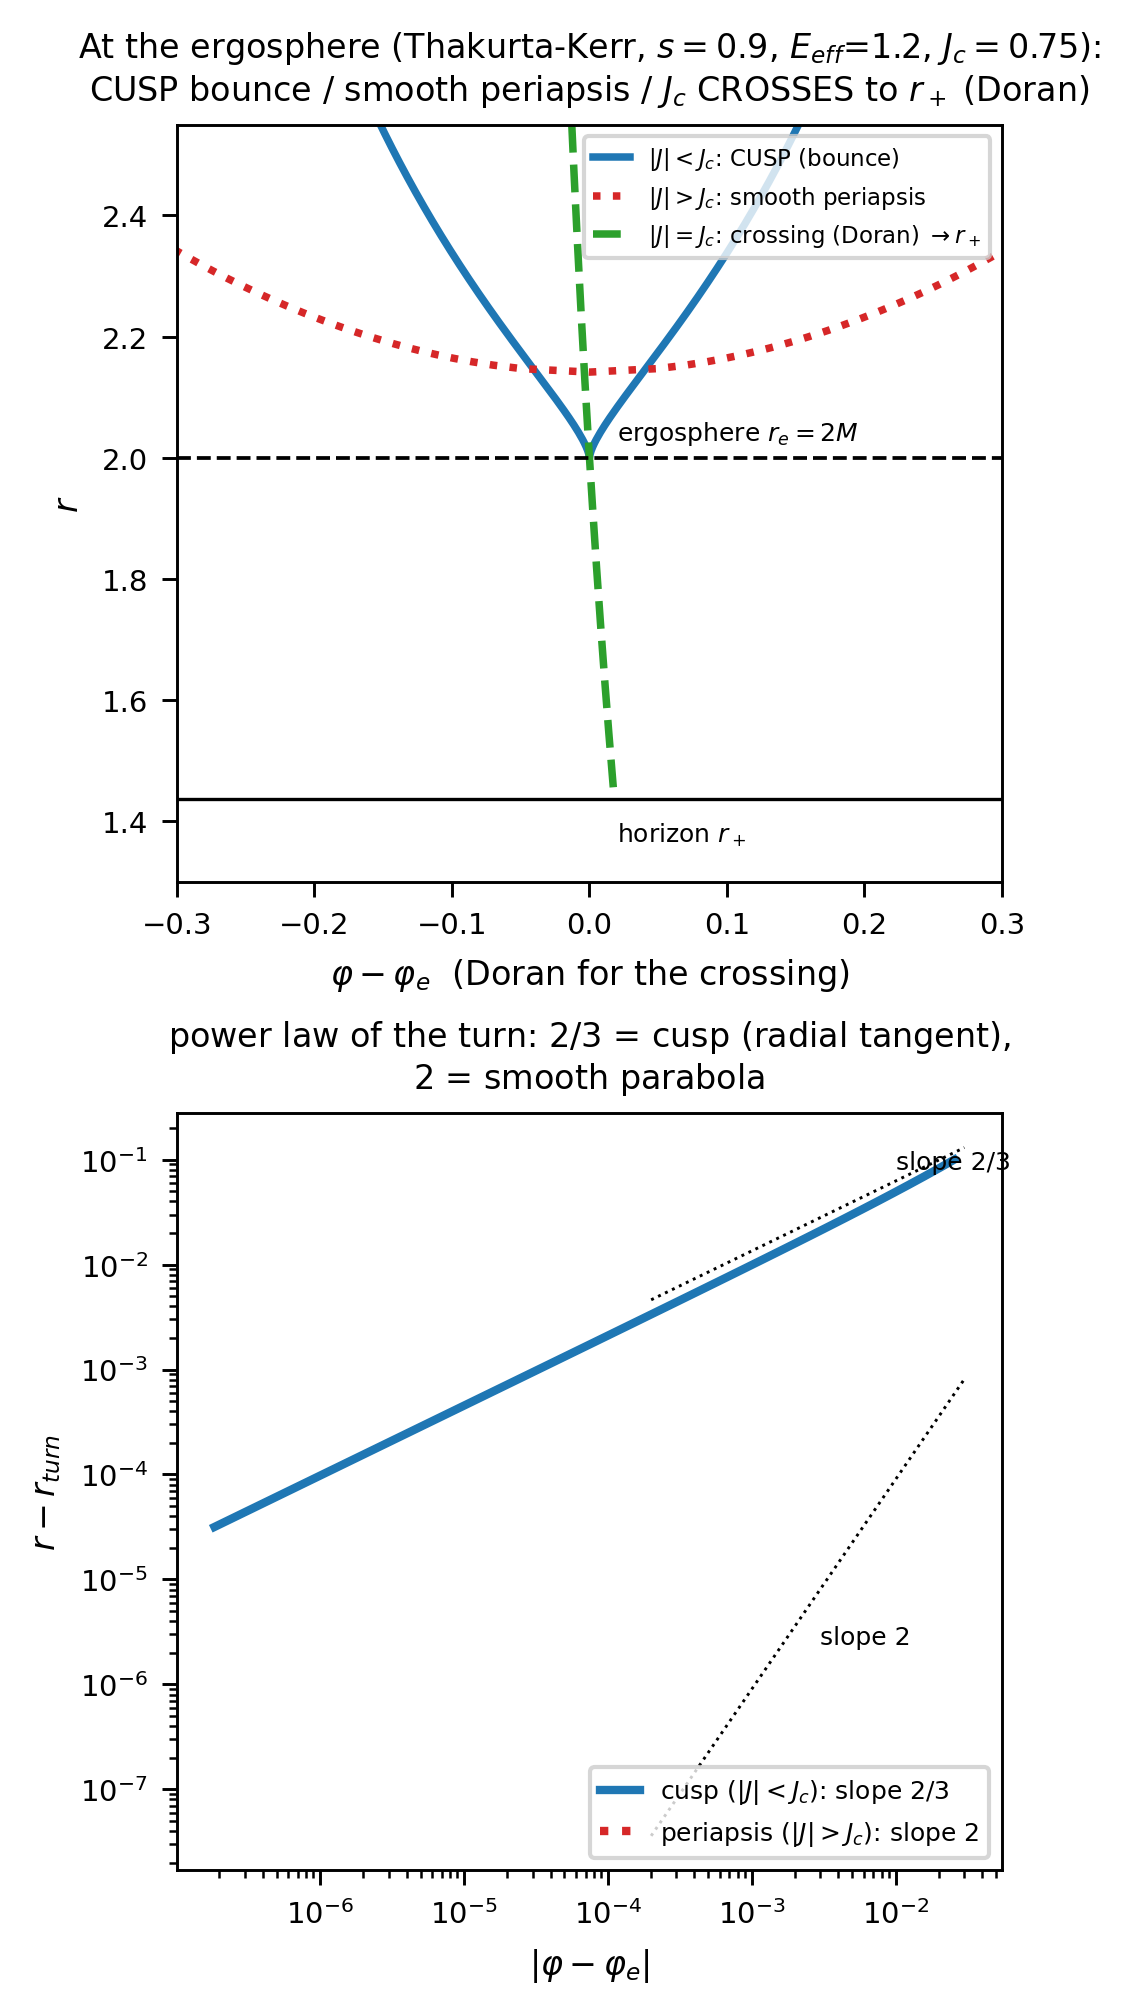
\includegraphics[width=\textwidth,height=0.68\textheight,keepaspectratio]{Immagini/fig_thakurta_cuspide_ergosfera.png}
    \caption{Reflection at the ergosphere: cusp ($|J|<\Jc$), smooth crossing
    to $\rp$ in Doran coordinates ($|J|=\Jc$), smooth periapsis
    ($|J|>\Jc$); power law $2/3$ vs $2$.}
    \label{fig:th-cusp}
\end{figure}

\subsection{Plunge inversion: rotational and conformal}
\label{sec:inversion}
Two mechanisms invert the $t/\tau$ ordering. Rotationally, in the $(a,J)$ plane,
$\rho(r_*)^2=H_{t0}/H_{\tau0}$, extending the stationary Kerr analysis
\cite{RosignoliKerr}. Conformally, the inversion locus is
\begin{equation}
    \mathrm{cond}(r,A)=A^2 b\,Q-\bar P(\Ehat-A^2 f)=0,\quad
    Q=b\bar v^2+\sqrt{\bar v^2\Delta},
    \label{eq:condinv}
\end{equation}
with $\mathrm{cond}(1)<0$ and
$\mathrm{cond}(\Af)=\Ehat r\Delta(\Ehat-1)/(r-2M)>0$, so by the intermediate
value theorem $A_{\rm inv}\in(1,\Af)$: the conformal inversion always exists
and is reachable (far field $A_{\rm inv}\to\sqrt{\Ehat}$).

\begin{figure}[ht]
    \centering
    
\includegraphics[width=\textwidth,height=0.68\textheight,keepaspectratio]{Immagini/fig_thakurta_kerr_plunge_t_tau.png}
    \caption{Rotational inversion in the $(a,J)$ plane; ODE locus vs analytic
    $\rho(r_*)^2=H_{t0}/H_{\tau0}$.}
    \label{fig:th-plungeAJ}
\end{figure}

\begin{figure}[tbp]
    \centering
    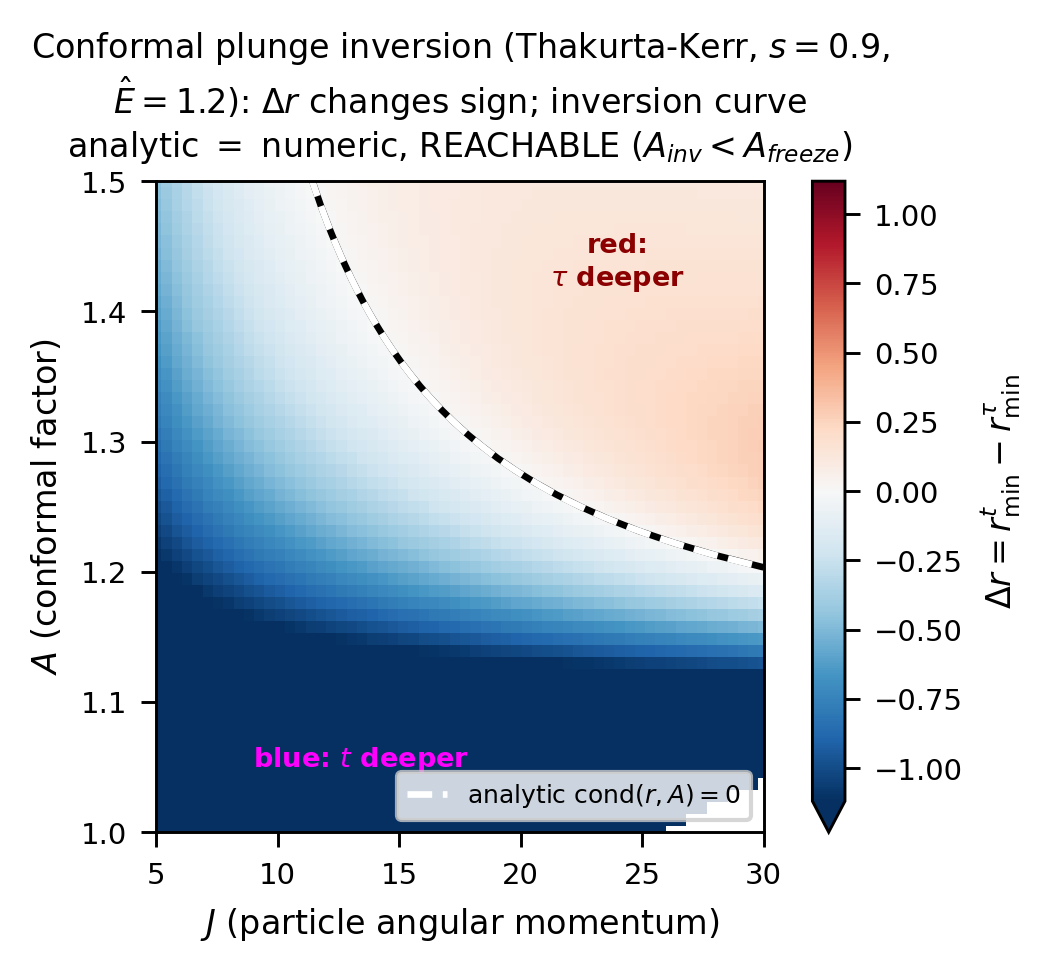
\includegraphics[width=\textwidth,height=0.68\textheight,keepaspectratio]{Immagini/fig_thakurta_kerr_inversione_AJ.png}
    \caption{Conformal inversion in the $(J,A)$ plane: $\Delta r$ changes sign;
    analytic $\mathrm{cond}=0$ matches the numerical contour; reachable
    ($A_{\rm inv}<\Af$).}
    \label{fig:th-invAJ}
\end{figure}


\subsection{Fixed-endpoint comparison and protocol dependence}
\label{sec:bvp}
The statement ``branch $X$ plunges deeper'' is protocol dependent. With
\emph{fixed initial data} (same $r_0,J,p_r$) the $t$-branch is deeper
($r_{\min}^t<r_{\min}^\tau$). With \emph{fixed endpoints} (the genuine
two-point brachistochrone), the two branches join the same $A,B$ but are
distinct paths, and the ordering reverses: $r_{\min}^\tau<r_{\min}^t$. The
optical-index ratio $n_t/n_\tau=E/f>1$ penalizes deep radii more heavily for
the $t$-branch, so the $t$-brachistochrone bows outward while the $\tau$-branch
dips. This must be specified when comparing depths.

\begin{figure}[ht]
    \centering
    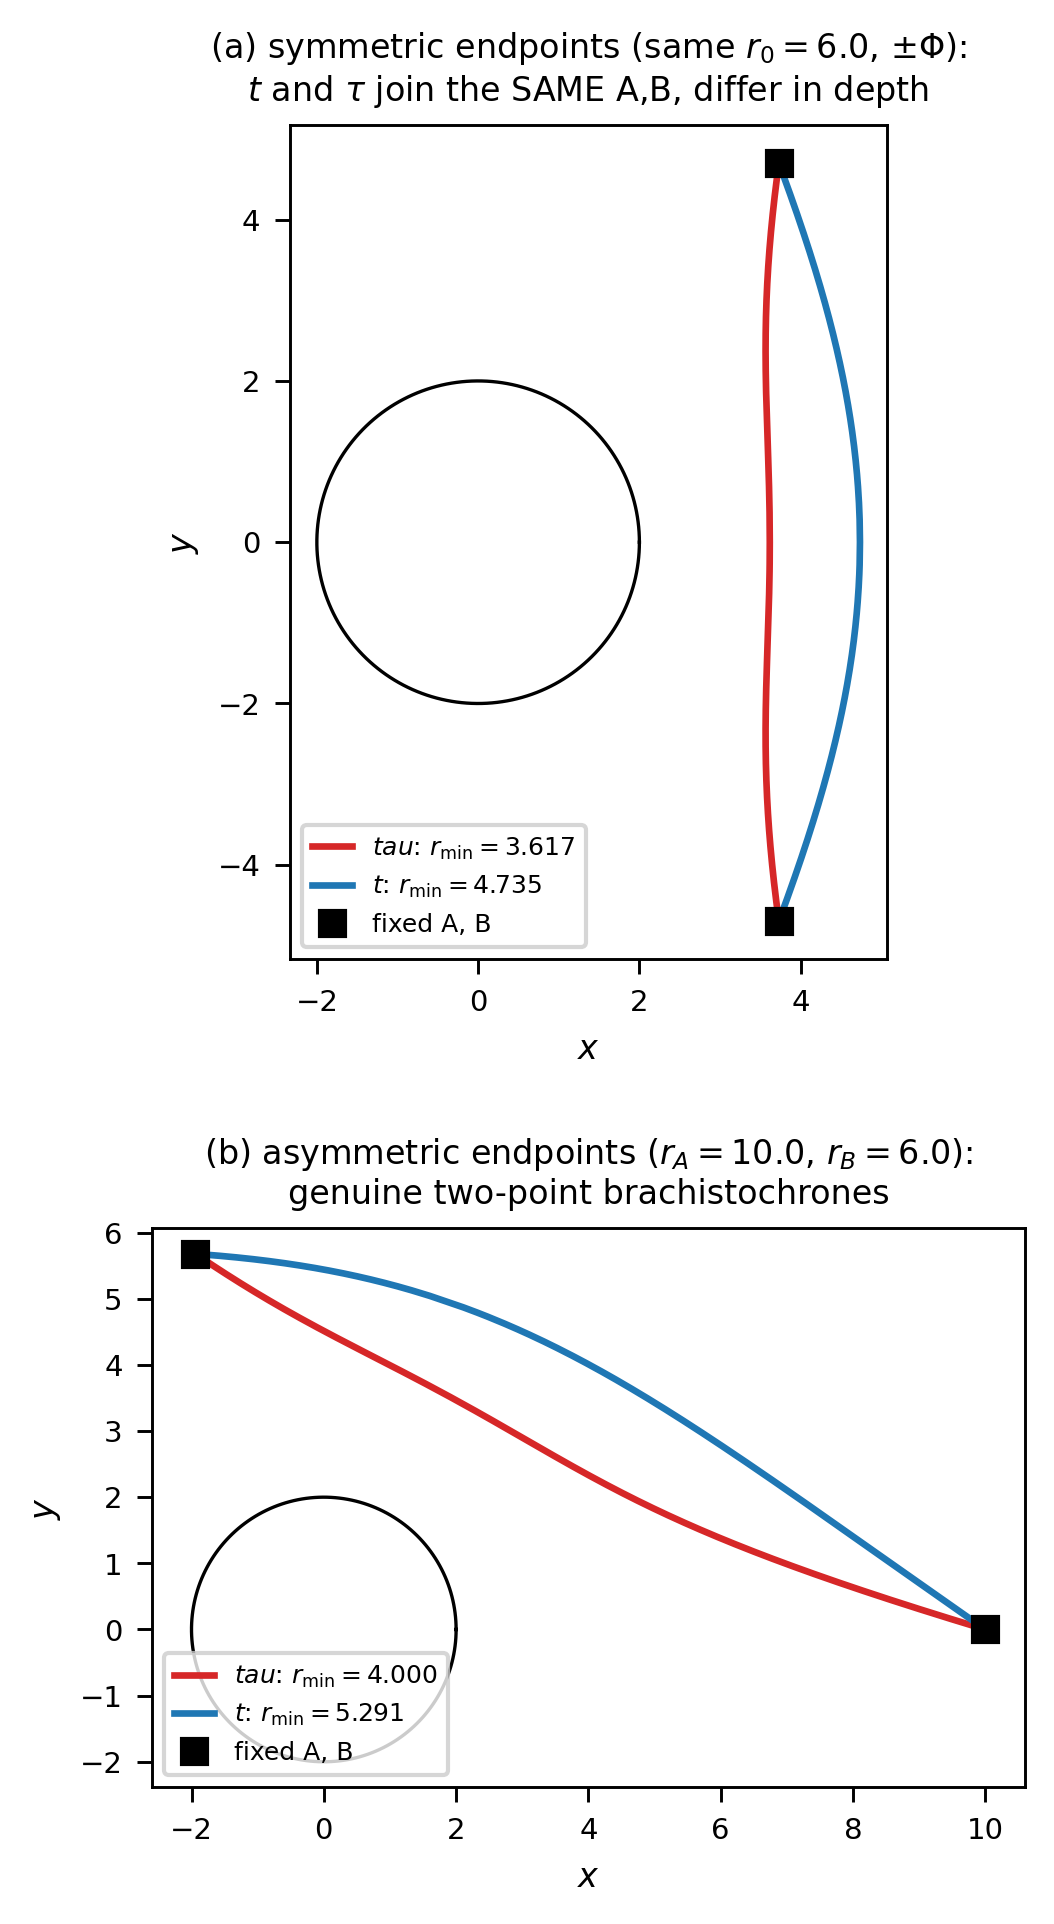
\includegraphics[width=\textwidth,height=0.68\textheight,keepaspectratio]{Immagini/fig_bvp_estremi_fissi.png}
    \caption{Fixed-endpoint $t$ and $\tau$ brachistochrones (Schwarzschild,
    $E=1.2$): symmetric (top) and asymmetric (bottom) endpoints. Both branches
    join the same $A,B$; the $\tau$-branch dips deeper.}
    \label{fig:bvp}
\end{figure}

Crucially, neither driver of same-launch inversion survives the
fixed-endpoint constraint. Scanning the spin $a$ over the entire
Kerr flow with fixed symmetric endpoints $(r_0,\pm\Phi)$ leaves
$\Delta r=r_{\min}^t-r_{\min}^\tau$ strictly positive
($\Delta r\in[+0.45,+2.06]$ on $a\in[0.05,0.95]$); the map is nearly flat
in $a$, its gradient set almost entirely by the endpoint angle
$\Phi$ (encoded by $J$). The conformal scan (via the transfer
$E_{\rm eff}=\hat E/A$) is likewise everywhere positive
($\Delta r\in[+0.002,+3.711]$), as forced by the theorem $n_t/n_\tau=E/f>1$.
Table~\ref{tab:protocol} summarizes the resulting protocol dependence:
inversion is a property of the \emph{comparison protocol}, not an invariant
of the two brachistochrones---it requires the freedom to let the endpoint
move.

\begin{figure}[tbp]
    \centering
    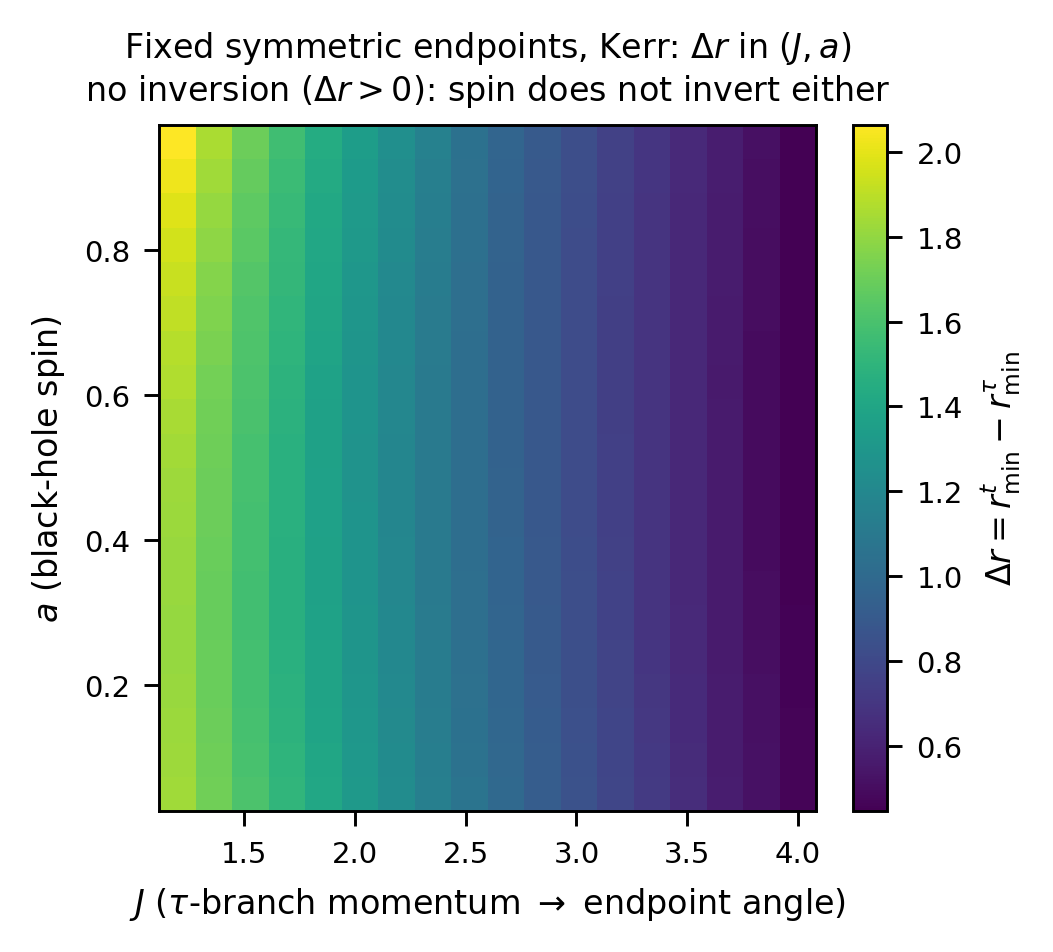
\includegraphics[width=\textwidth,height=0.68\textheight,keepaspectratio]{Immagini/fig_colormap_spin_estremi_fissi.png}
    \caption{Spin scan at fixed symmetric endpoints (Kerr, Hamiltonian
    flow): $\Delta r$ in the $(J,a)$ plane stays positive everywhere---spin
    does not invert once the endpoints are pinned. The gradient is set by the
    endpoint angle ($J$), not by $a$.}
    \label{fig:cm-spin-fix}
\end{figure}


The verdict is independent of the endpoint symmetry: repeating both scans
with \emph{asymmetric} fixed endpoints ($r_A=10,r_B=6$) leaves
$\Delta r>0$ everywhere as well (spin $[+0.76,+2.64]$, conformal
$[+0.16,+3.24]$; Figs.~\ref{fig:asym-spin}--\ref{fig:asym-conf}),
consistent with the pointwise bound $n_t/n_\tau=E/f$.

\begin{table}[t]
    \centering
    \caption{Protocol dependence of plunge inversion. Same-launch
    comparison inverts under either rotation or a conformal factor;
    the genuine fixed-endpoint brachistochrone never inverts.}
    \label{tab:protocol}
    \begin{tabular}{@{}lcc}
        \br
        protocol & spin $a$ & conformal $A$ \\
        \mr
        same launch & inverts (\S\ref{sec:inversion}) & inverts (\S\ref{sec:inversion}) \\
        fixed endpoints & no ($\Delta r>0$) & no ($n_t/n_\tau=E/f>1$) \\
        \br
    \end{tabular}
\end{table}


% ======================================================================
\section{Conclusions}
\label{sec:concl}
% ----------------------------------------------------------------------
The non-stationary brachistochrone is a well-posed controlled-rail problem: the
invariant $-u\cdot W=\Ehat$ is legitimate via Pontryagin's principle, and the
selector $W$ is fixed canonically by the Killing--CKV--Kodama hierarchy, with
the Kodama energy conserved along the rail even when free fall does not conserve
it. FLRW is the degenerate base---freezing without branch splitting---while the
mass breaks the $t/\tau$ symmetry through its radial gravitational gradient (the
spin instead driving the rotational plunge inversion). On
the equatorial sector we obtained closed-form separatrices in Weierstrass
functions, continued through the ergosphere in Doran coordinates, and an analytic
cusp theorem for the $|J|<\Jc$ reflection. The plunge inversion resolves into a
three-way picture: rotation and the conformal factor invert the $t/\tau$
ordering under a same-launch comparison, whereas physical evaporation never does,
and \emph{no} inversion survives once both endpoints are fixed. Outlook: the
exact Sultana--Dyer source
\cite{SultanaDyer2005}, the McVittie/Schwarzschild--de Sitter limits
\cite{McVittie1933,Kottler1918,Kaloper2010} with their photon surfaces
\cite{ClaudelViracVirbhadra2001}, escape maps, and freezing-surface dynamics.

\ack
The author thanks the University of Pavia for providing a stimulating academic
environment. The author received no external funding for this work. The AI
assistants GPT~5.5 (OpenAI) and Claude Fable (Anthropic) were used to assist with
symbolic derivations, numerical implementation, and manuscript preparation; all
results were verified independently by the author, who takes full responsibility
for the content of this work.

\section*{Data availability}
The complete numerical and symbolic codebase underlying this work is openly
available under the MIT license in the GitHub repository
``NonStationary\-Brachi\-sto\-chrone''~\cite{Rosignoli2026Code}:
\begin{center}
\url{https://github.com/ImanetorX98/NonStationaryBrachistochrone}
\end{center}
The repository includes the trajectory integrators, the Pontryagin Hamiltonian
constructions, the Poisson-bracket closure and quasi-invariant scans
(Sec.~\ref{sec:quasiconst}), the Weierstrass separatrix and Doran-continuation
scripts, the fixed-endpoint BVP and colormap pipelines, and the
figure-generation code. It also retains exploratory scripts and negative results,
documenting which ansatz classes failed the held-out trajectory and phase-space
residual tests reported in Sec.~\ref{sec:quasiconst} and
App.~\ref{app:validation}.



% ======================================================================
\appendix
\section{Validation and consistency checks}
\label{app:validation}
We collect the numerical checks that underpin the analytic results. The
minimum principle is verified directly by perturbing the computed
brachistochrones and confirming that both $T_t$ and $T_\tau$ are minimized
(Fig.~\ref{fig:flrw-var} for the FLRW branch degeneracy, and
Fig.~\ref{fig:verifmin} for the two distinct Vaidya branches). Stationary-limit
residuals confirm that the non-stationary
Hamiltonian flow reproduces the closed-form Kerr expressions as $m'\to0$ and
$A\to1$ (Fig.~\ref{fig:vaidya-kerra0}); the Kodama energy is conserved to
$\sim10^{-16}$ along the rail (Fig.~\ref{fig:kodama}). The equatorial closed
forms are validated end-to-end by the three-method superposition
(ODE flow, quadrature, evaluated Weierstrass) through the ergosphere
(Fig.~\ref{fig:sep3}), and the fixed-endpoint no-inversion theorem is
checked over the asymmetric-endpoint grids (Figs.~\ref{fig:asym-spin}--%
\ref{fig:asym-conf}).

\subsection{Explicit closed forms}
\label{app:explicit}

\paragraph{Equatorial $\tau$-branch separatrix in Weierstrass functions.} On the
$\tau$-separatrix $J=\Jc$ the doranTau factorization $\Delta-\Jc^2 w=f(r^2+c^2)$,
$c=a/E$, makes the
turning quartic $Q_4=r\big((E^2-1)r+2M\big)(r^2+c^2)$, and the factor $r^2+c^2$
divides $Q_4$ so that only the horizon poles survive. Writing
\begin{gather}
    A=\frac{Ma^2}{2E^2},\qquad B=\frac{a^2(E^2-1)}{12E^2},\notag\\
    g_2=\frac{a^4(E^2-1)^2}{12E^4}-\frac{a^2M^2}{E^2},\notag\\
    g_3=\frac{a^4\big[36E^2M^2(1-E^2)-a^2(E^2-1)^3\big]}{216E^6},
    \label{eq:wp-invariants}
\end{gather}
the uniformizing variable is $z(r)=\wp^{-1}\!\big(A/r+B;g_2,g_3\big)
=\int_0^r\dd r'/\sqrt{Q_4}$, the Abel map of the turning quartic $Q_4$: it is the
elliptic argument in which the radial motion linearizes, so that $r$ is recovered
by $A/r+B=\wp(z)$ and the physical range $r\in[r_{\min},\infty)$ maps to a
segment of $z$. With $r_\pm=M\pm\sqrt{M^2-a^2}$ the horizons,
\begin{equation}
\begin{aligned}
    \alpha_\pm&=\frac{r_\pm\big((E^2-1)r_\pm+2M\big)}{r_\pm-r_\mp},\\
    \lambda_\pm&=\frac{\alpha_\pm}{\sqrt{Q_4(r_\pm)}},\qquad v_\pm=z(r_\pm),
\end{aligned}
\end{equation}
$\wp(v_\pm)=A/r_\pm+B$, and
$\Lambda_0=(E^2-1)-\alpha_+/r_+-\alpha_-/r_-+2\lambda_+\zeta(v_+)+2\lambda_-\zeta(v_-)$,
the angle is linear in the uniformizing variable $z\equiv z(r)$ plus two
Weierstrass-$\sigma$ ratios,
\begin{equation}
\begin{split}
    \varphi(r)=\frac{a}{E}\Big[&\Lambda_0\,z(r)
      +\lambda_+\ln\frac{\sigma(z-v_+)}{\sigma(z+v_+)}\\
      &+\lambda_-\ln\frac{\sigma(z-v_-)}{\sigma(z+v_-)}\Big]+\text{const}.
\end{split}
    \label{eq:sep-phi}
\end{equation}
Because $Q_4(2M)=4M^2(4E^2M^2+a^2)>0$, Eq.~\eqref{eq:sep-phi} is regular
\emph{through} the ergosphere $\re=2M$; the only singularities are the
third-kind logarithms at the horizons. The conformal case is
$E\to E_{\rm eff}=\Ehat/A$ in every parameter.

\paragraph{Doran continuation through the horizon.} The Boyer--Lindquist form
$\varphi(r)$ winds logarithmically at $\rp$ (the standard BL artifact); adding the
Doran shift $\dd\varphi_{\rm shift}=2Mar\,\dd r/(\Delta\sqrt{C_3})$ with the cubic
$C_3=2Mr(r^2+a^2)$ regularizes it. This is a \emph{second} elliptic curve, in
clean Weierstrass form $r(z)=(2/M)\wp(z;g_2,g_3)$ with $g_2=-M^2a^2$, $g_3=0$
(quasi-lemniscatic), giving
$\varphi_{\rm shift}=\tfrac{a}{r_+-r_-}\big(B_+-B_-\big)$,
$B_\pm=2\zeta(v_\pm)z+\ln[\sigma(z-v_\pm)/\sigma(z+v_\pm)]$; the log divergences of
$\varphi$ and $\varphi_{\rm shift}$ cancel at $\rp$, the analytic content of Doran
regularity. Thus $\varphi_D=\varphi_{\rm BL}+\varphi_{\rm shift}$ is closed on two
elliptic curves.

\paragraph{$t$-branch separatrix in Weierstrass functions.} The coordinate-time
brachistochrone has $\dd\varphi/\dd r=\mathcal K(r)/\sqrt{\mathcal R(r)}$ with the
\emph{sextic} radical $\mathcal R=r\,Q_2(r)\,[(E^2-1)r+2M]$ ($Q_2$ quartic),
genus~2. At the saddle-node $J_c^-$ [Eq.~\eqref{eq:Jc-minus}] it acquires a
\emph{double root} at the marginal-capture radius $r_*$,
$\mathcal R=(r-r_*)^2 Q_4(r)$, and
$\dd\varphi/\dd r=\mathcal G(r)/\sqrt{Q_4}$ becomes a third-kind elliptic
differential on the quartic $Q_4$ (which retains the root $r=0$). With the same
uniformization $z(r)=\wp^{-1}(A/r+B;g_2,g_3)$ (invariants of $Q_4$) the closed
form is
\begin{equation}
    \varphi(r)=\Lambda_0\,z(r)+\sum_{k}\lambda_k\,
      \ln\frac{\sigma(z-v_k)}{\sigma(z+v_k)},
    \label{eq:t-sep-phi}
\end{equation}
now with third-kind poles only at $c_k\in\{\rp,\rm,r_*\}$---three real ones, with
\emph{no} pole at $r=0$ and no complex pair, unlike the $\tau$-separatrix. Here
$v_k=\wp^{-1}(A/c_k+B)$, $\lambda_k=-A\alpha_k/(c_k^2\wp'(v_k))$, and
$\Lambda_0=\Lambda_{\rm poly}-\sum_k\alpha_k/c_k+\sum_k 2\zeta(v_k)\lambda_k$,
with $\alpha_k$ the residues of $\mathcal G$. For $M=1$, $a=0.9$, $E=1.2$
($r_*=3.514$, $J_c^-=-8.05$) Eq.~\eqref{eq:t-sep-phi} reproduces the Hamiltonian
flow to $2\times10^{-14}$ (Fig.~\ref{fig:t-sep}). So both separatrices are
genus~1 by different mechanisms; only non-separatrix $t$-orbits need genus-2
Kleinian functions.

\begin{figure}[ht]
    \centering
    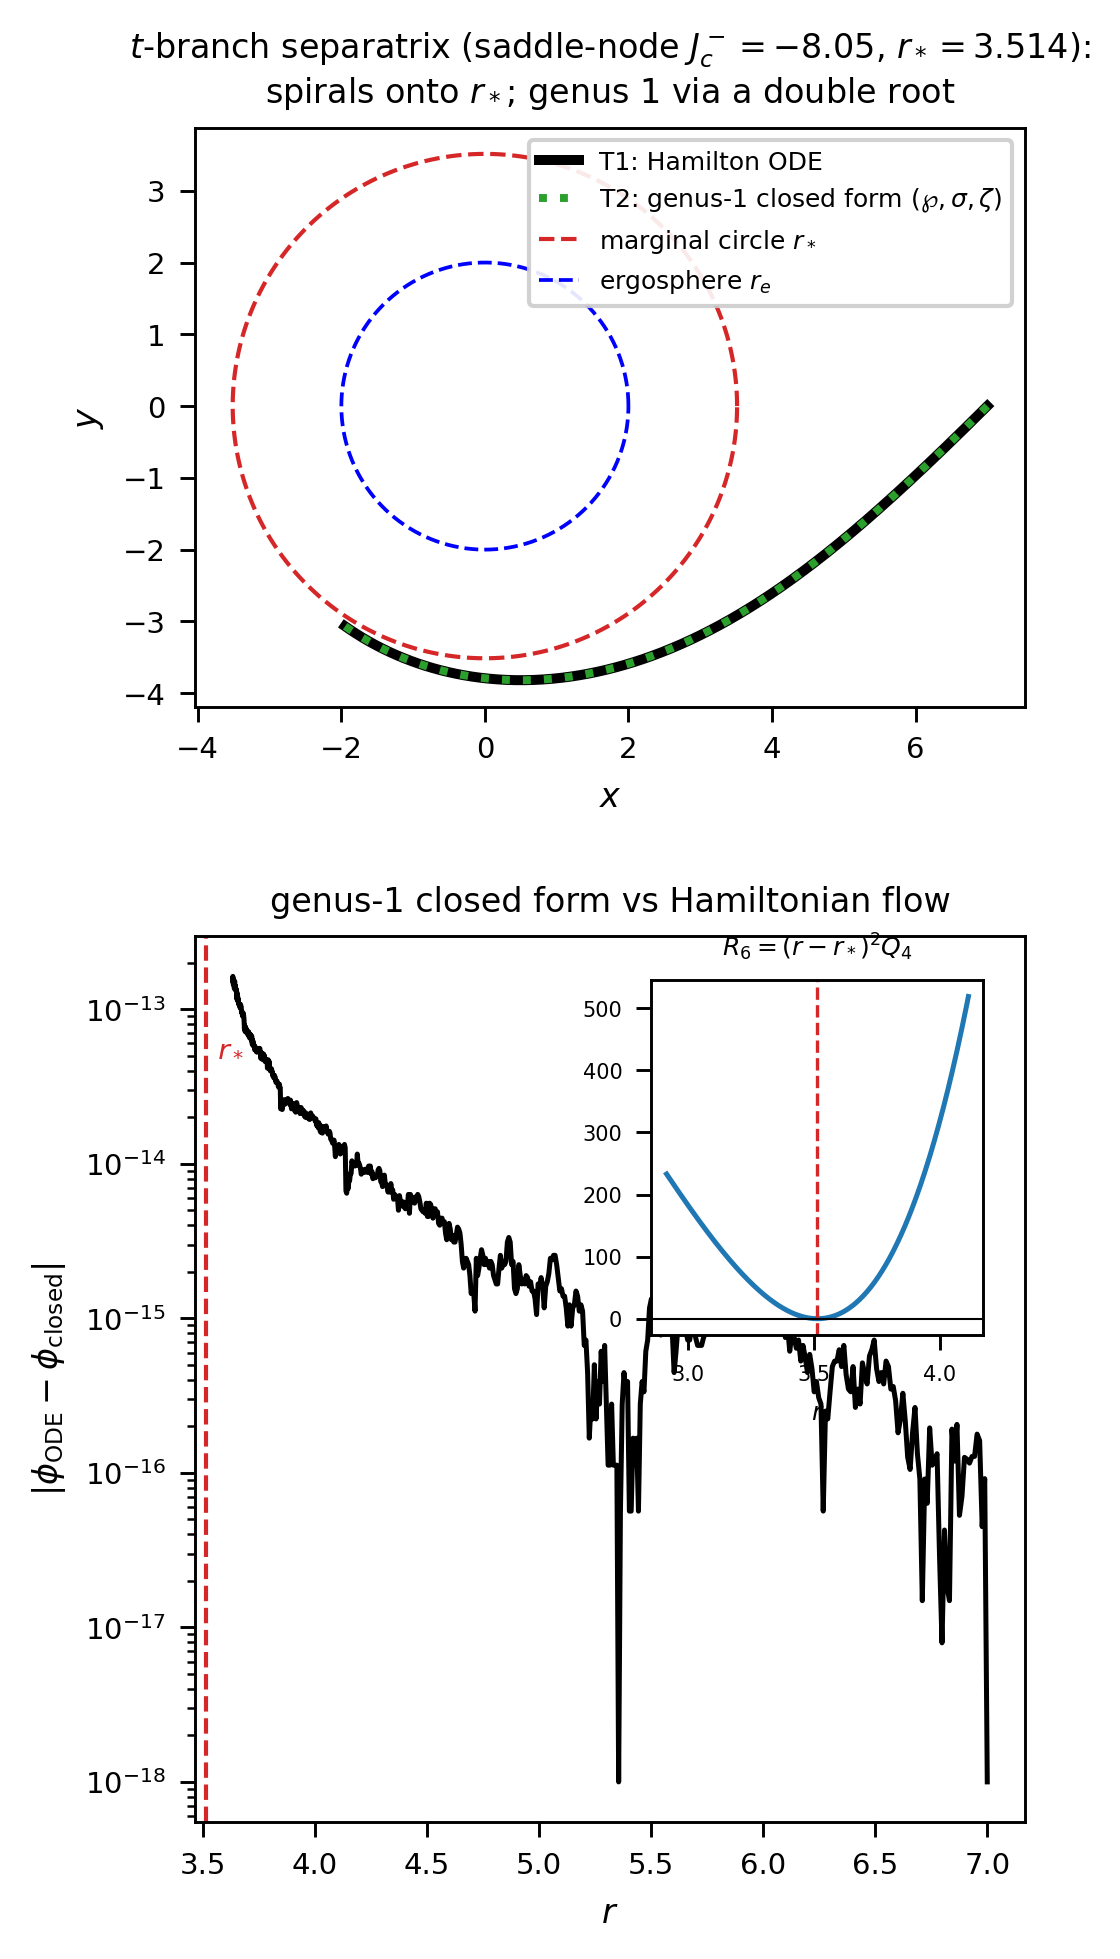
\includegraphics[width=\textwidth,height=0.68\textheight,keepaspectratio]{Immagini/fig_tbranch_separatrix.png}
    \caption{$t$-branch separatrix (the retrograde saddle-node $J_c^-$): the
    orbit spirals onto the marginal circle $r_*$. Top: Hamilton ODE vs the
    genus-1 closed form (the sextic radical has a double root, dropping to the
    quartic $Q_4$). Bottom: they agree to $\sim10^{-13}$; inset shows the double
    root of $R_6=(r-r_*)^2Q_4$.}
    \label{fig:t-sep}
\end{figure}

\paragraph{Stationary-limit conserved quantities.} At $A=1$ the branch flows admit
the closed first integrals used for validation,
\begin{equation}
    \mathcal K_\tau=J,\qquad
    \mathcal K_t=\frac{fJ+2Ms/r}{E},\qquad
    \mathcal K_\eta=\frac{fJ}{E},
    \label{eq:kerr-conserved}
\end{equation}
the equatorial Kerr doranTau/doranT constants.

\paragraph{Rotational inversion function.} The same-launch $t/\tau$ ordering
inverts where $\rho(r_*)^2=H_{t0}/H_{\tau0}$ with the explicit ratio of
centrifugal potentials
\begin{equation}
    \rho=\frac{A^2}{\Ehat}\Big(f+\frac{2Ms}{rJ}\Big),
    \label{eq:rho-explicit}
\end{equation}
$\rho<1$ giving $t$ deeper, $\rho>1$ giving $\tau$ deeper.

\paragraph{Conformal trichotomy.} With constant $A$ the separatrix momentum is
$\Jc=sA^2/\Ehat$, and above it the smooth periapsis is the outer root of
\begin{equation}
    \Delta(r)-\Big(\tfrac{J}{A}\Big)^2\Big[\big(\tfrac{\Ehat}{A}\big)^2-f(r)\Big]=0,
    \label{eq:periapsis-root}
\end{equation}
while $|J|<\Jc$ reflects at the cusp $r_{\min}=\re$ and $|J|=\Jc$ crosses to
$\rp$.

\paragraph{Closed toroidal averages.} The secular source $\langle S_1\rangle$ of
Eq.~\eqref{eq:S1} follows from the orbit-plane averages ($\cos\theta=\sin i\,
\sin\psi$, $k=1-J^2/L^2$)
\begin{equation}
    \Big\langle\cos^2\theta\Big\rangle=\tfrac{k}{2},\quad
    \Big\langle\tfrac{1}{\sin^2\theta}\Big\rangle=\tfrac{L}{|J|},\quad
    \big\langle p_\theta^2\big\rangle=L(L-|J|),
    \label{eq:averages}
\end{equation}
with $\langle\cos2\theta\,p_\theta^2\rangle=|J|(L-|J|)$.

\subsection{Consistency residuals}
\label{app:residuals}
The closed forms and reductions above were checked symbolically and numerically.
The Weierstrass separatrix~\eqref{eq:sep-phi} reproduces the direct quadrature to
$|\Delta\varphi|<2.8\times10^{-10}$ through the ergosphere, with the $\wp$-identity
satisfied to $9\times10^{-28}$ and the antiderivative to $30$ digits; the Doran
shift reduces to $1.1\times10^{-16}$. The non-autonomous Randers
data~\eqref{eq:randers-data} match the Kerr null Fermat metric to
$\sim10^{-14}$. The equatorial Thakurta--Kerr flow reproduces the $A=1$ Kerr
constants~\eqref{eq:kerr-conserved} to ten digits at $r=4,6,9$ ($a=0.9$, $E=1.2$),
and the $s\to0$ limit the Thakurta--Schwarzschild flow to $10^{-12}$; the $3+1$
Hamiltonian~\eqref{eq:H3d} reduces to the equatorial one exactly, and conserves
$L^2$ to $6\times10^{-13}$ at $a=0$. The Kodama energy is held to
$|{-}u\cdot K-\Ehat|<7\times10^{-16}$ along the rail, and the static
inversion/trichotomy colormap agrees with the analytic
contours~\eqref{eq:periapsis-root} to a relative $7\times10^{-12}$.

\begin{figure}[tbp]
    \centering
    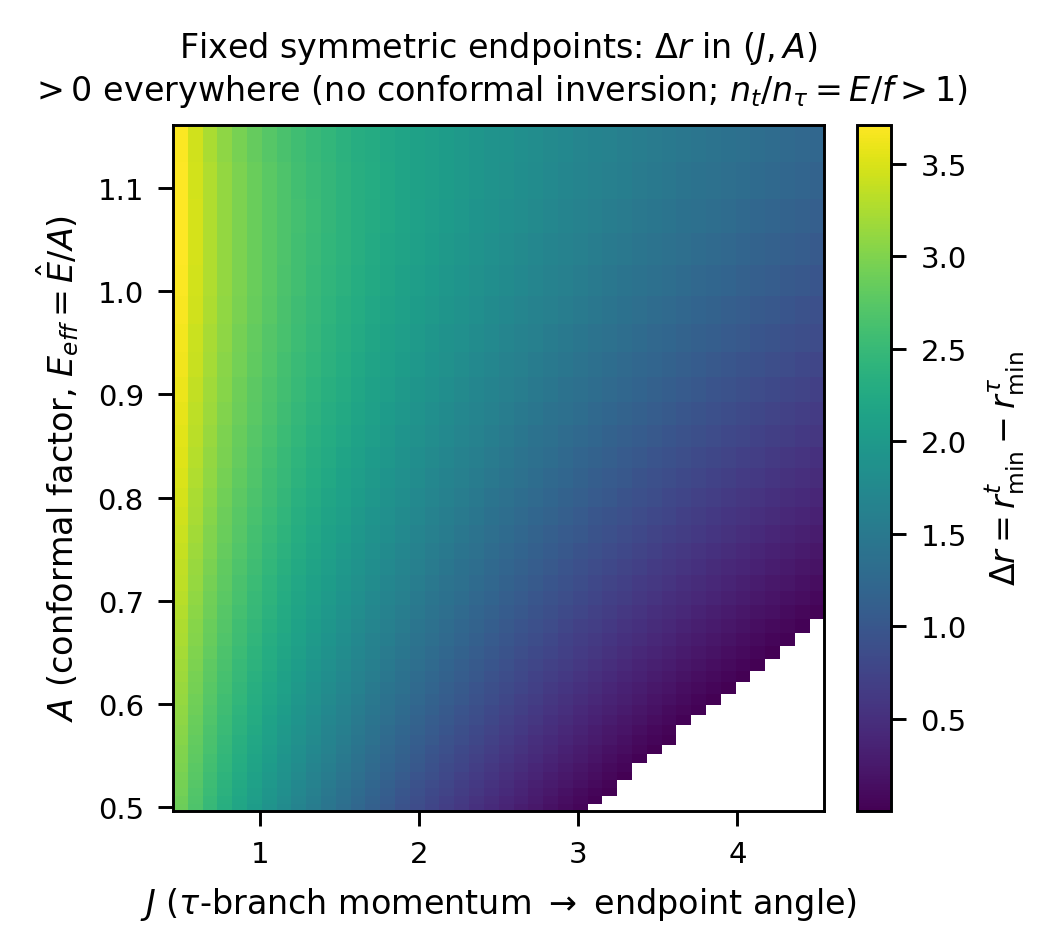
\includegraphics[width=\textwidth,height=0.68\textheight,keepaspectratio]{Immagini/fig_colormap_conforme_estremi_fissi.png}
    \caption{Conformal scan at fixed symmetric endpoints (via
    $E_{\rm eff}=\hat E/A$): $\Delta r$ in the $(J,A)$ plane is positive
    everywhere, matching the closed-form theorem $n_t/n_\tau=E/f>1$.}
    \label{fig:cm-conf-fix}
\end{figure}


\begin{figure}[tbp]
    \centering
    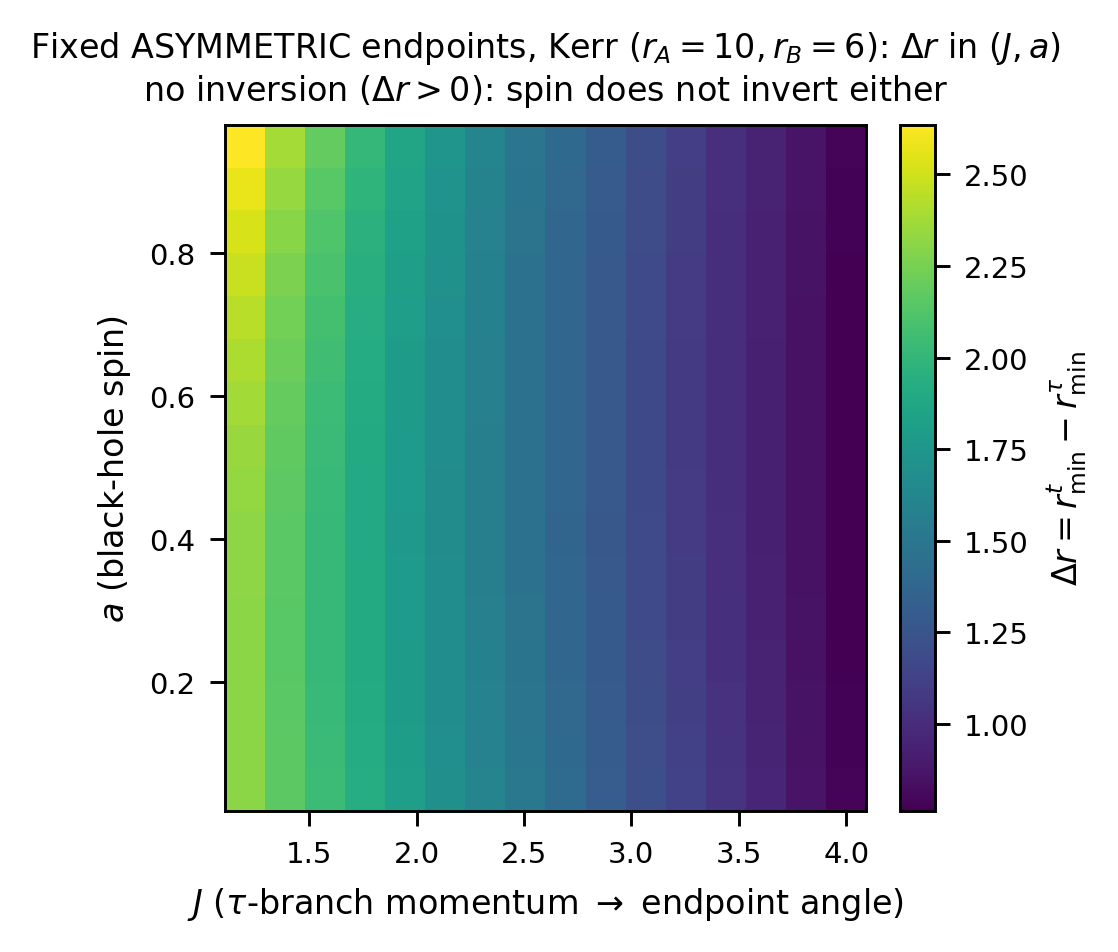
\includegraphics[width=\textwidth,height=0.68\textheight,keepaspectratio]{Immagini/fig_colormap_spin_asimmetrico.png}
    \caption{Robustness of the fixed-endpoint no-inversion result under
    \emph{asymmetric} endpoints ($r_A=10,r_B=6$), spin scan (Kerr flow):
    $\Delta r>0$ throughout the $(J,a)$ plane.}
    \label{fig:asym-spin}
\end{figure}

\begin{figure}[tbp]
    \centering
    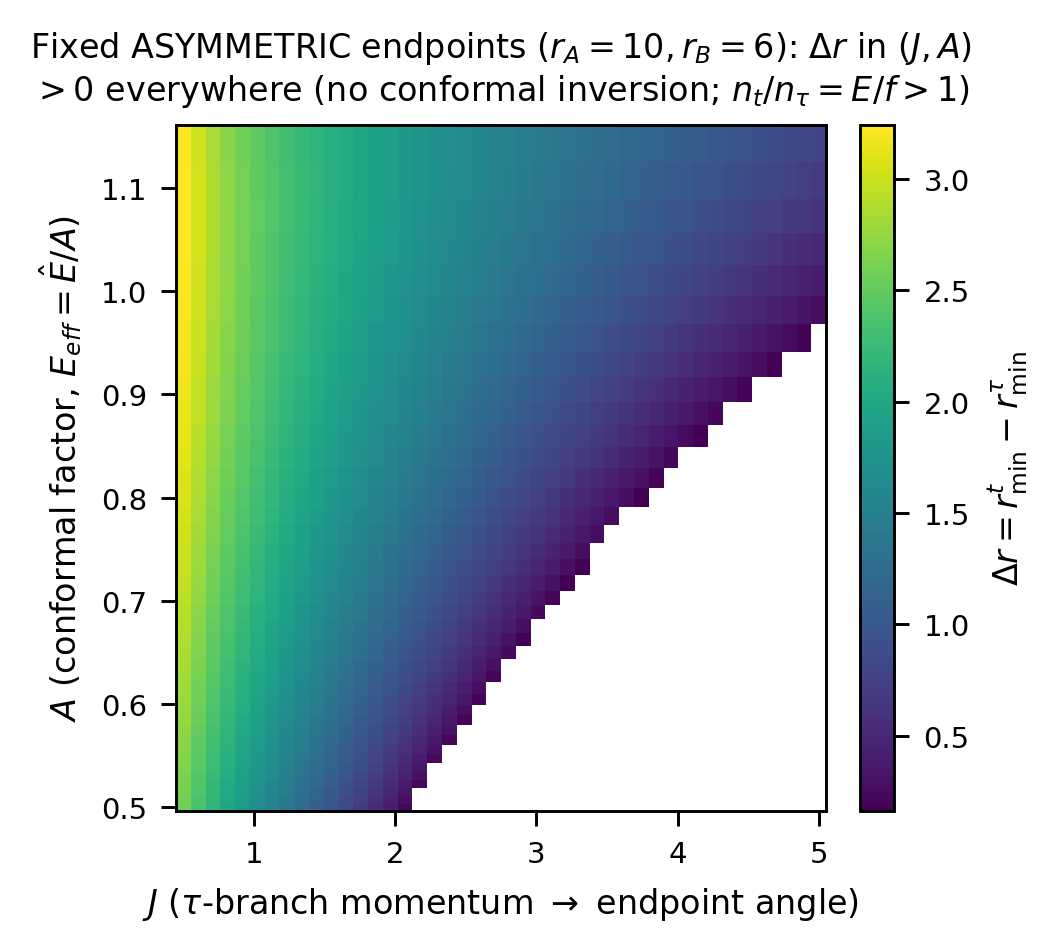
\includegraphics[width=\textwidth,height=0.68\textheight,keepaspectratio]{Immagini/fig_colormap_conforme_asimmetrico.png}
    \caption{Same robustness check, conformal scan (via $E_{\rm eff}=\hat E/A$):
    $\Delta r>0$ throughout the $(J,A)$ plane for asymmetric endpoints. The
    blank wedge is the region where the $\tau$-turning point rises above
    $r_B$ (no dipping orbit reaches $B$).}
    \label{fig:asym-conf}
\end{figure}

\clearpage

\begin{figure}[tbp]
    \centering
    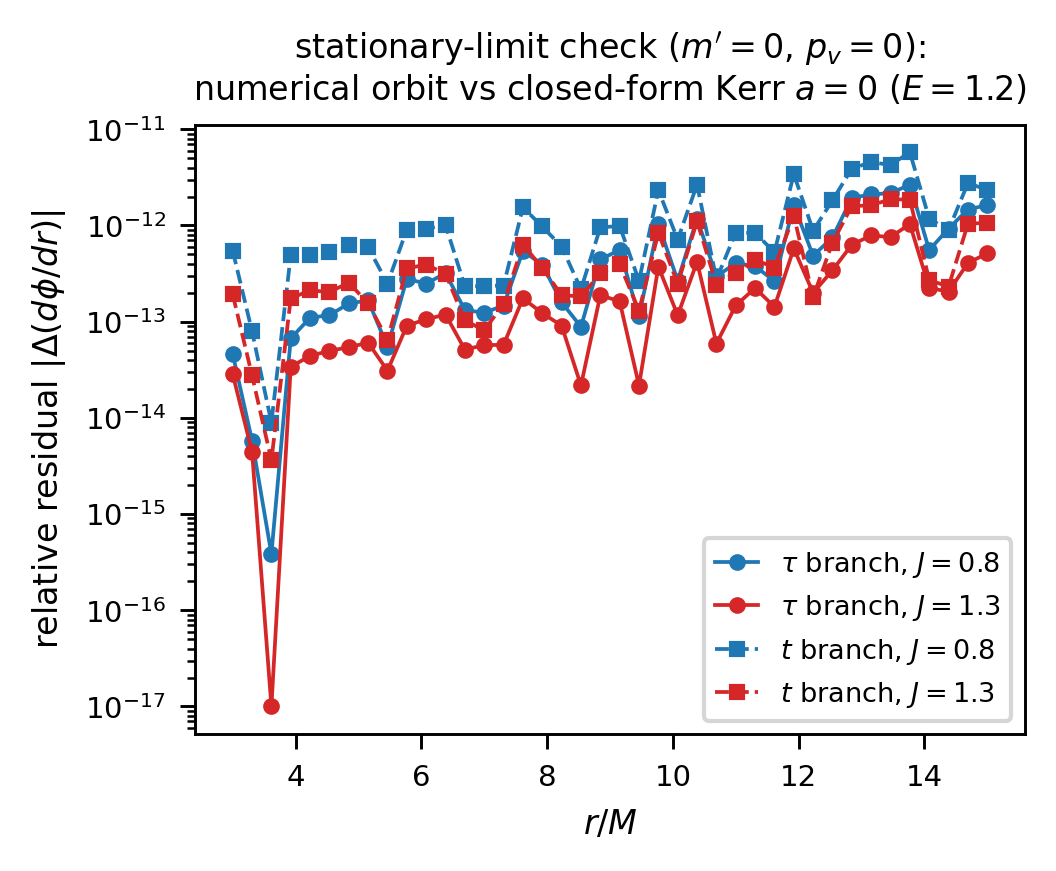
\includegraphics[width=\textwidth,height=0.68\textheight,keepaspectratio]{Immagini/fig_vaidya_kerr_a0.png}
    \caption{Stationary-limit check ($m'=0$): numerical orbit vs closed-form
    Kerr $a=0$.}
    \label{fig:vaidya-kerra0}
\end{figure}


\begin{figure}[tbp]
    \centering
    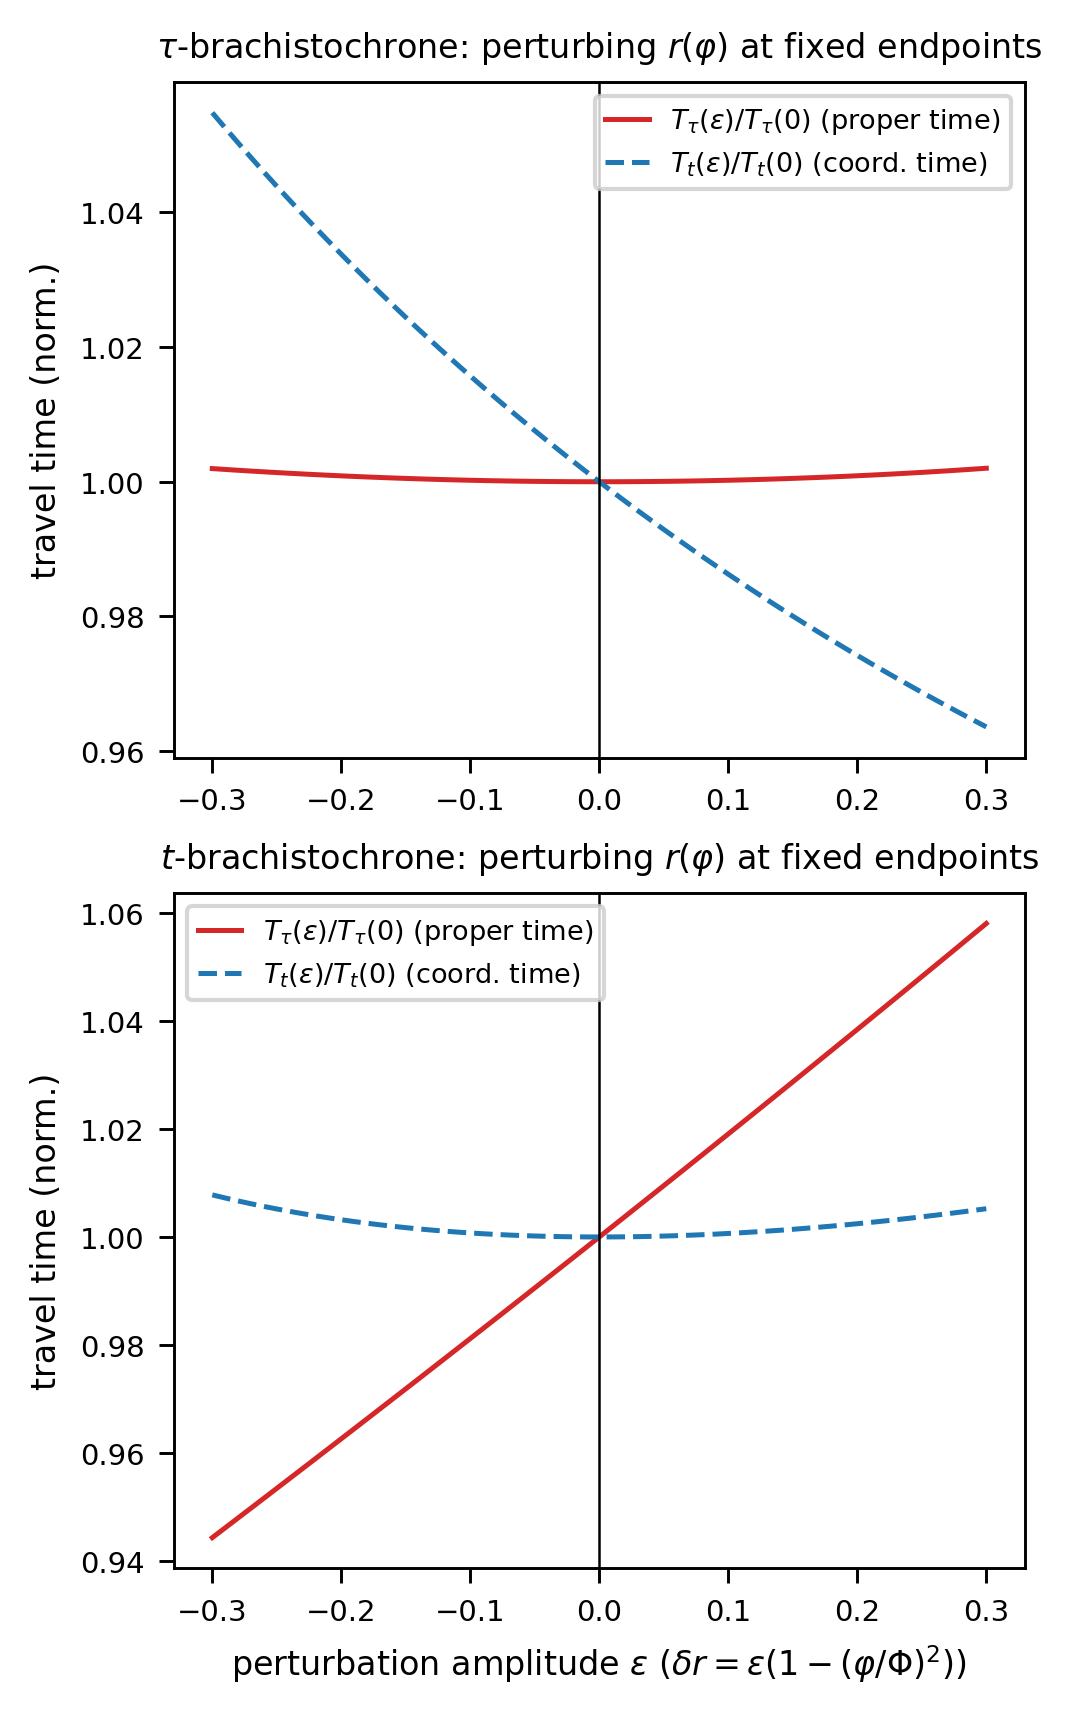
\includegraphics[width=\textwidth,height=0.68\textheight,keepaspectratio]{Immagini/fig_verifica_minimo_brachi.png}
    \caption{Each branch minimizes its own travel time; $t$ and $\tau$ are
    distinct curves.}
    \label{fig:verifmin}
\end{figure}

\begin{figure}[tbp]
    \centering
    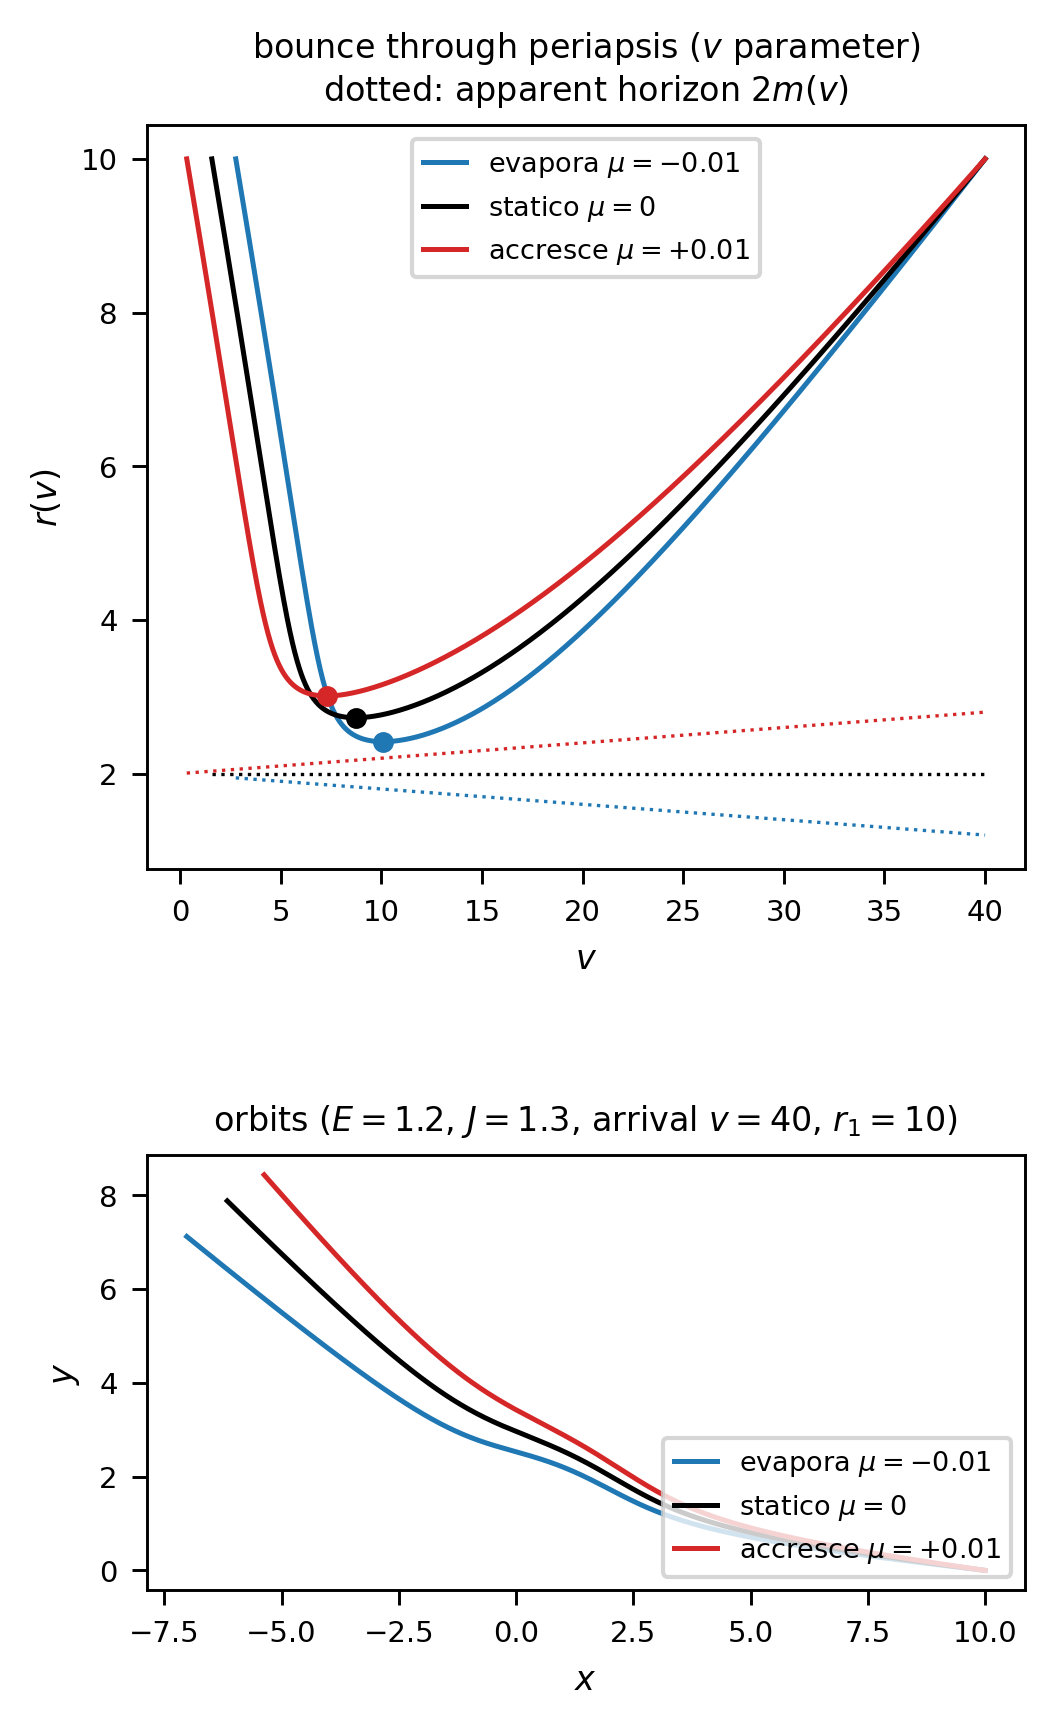
\includegraphics[width=\textwidth,height=0.68\textheight,keepaspectratio]{Immagini/fig_vaidya_bounce.png}
    \caption{Bounce through periapsis in the $v$-parametrization: the
    Euler--Lagrange flow is regular at $r'=0$ and integrates through the turning
    point, reaching $r_{\min}$ exactly where the $r$-parametrization diverges.}
    \label{fig:vaidya-bounce}
\end{figure}

\begin{figure}[tbp]
    \centering
    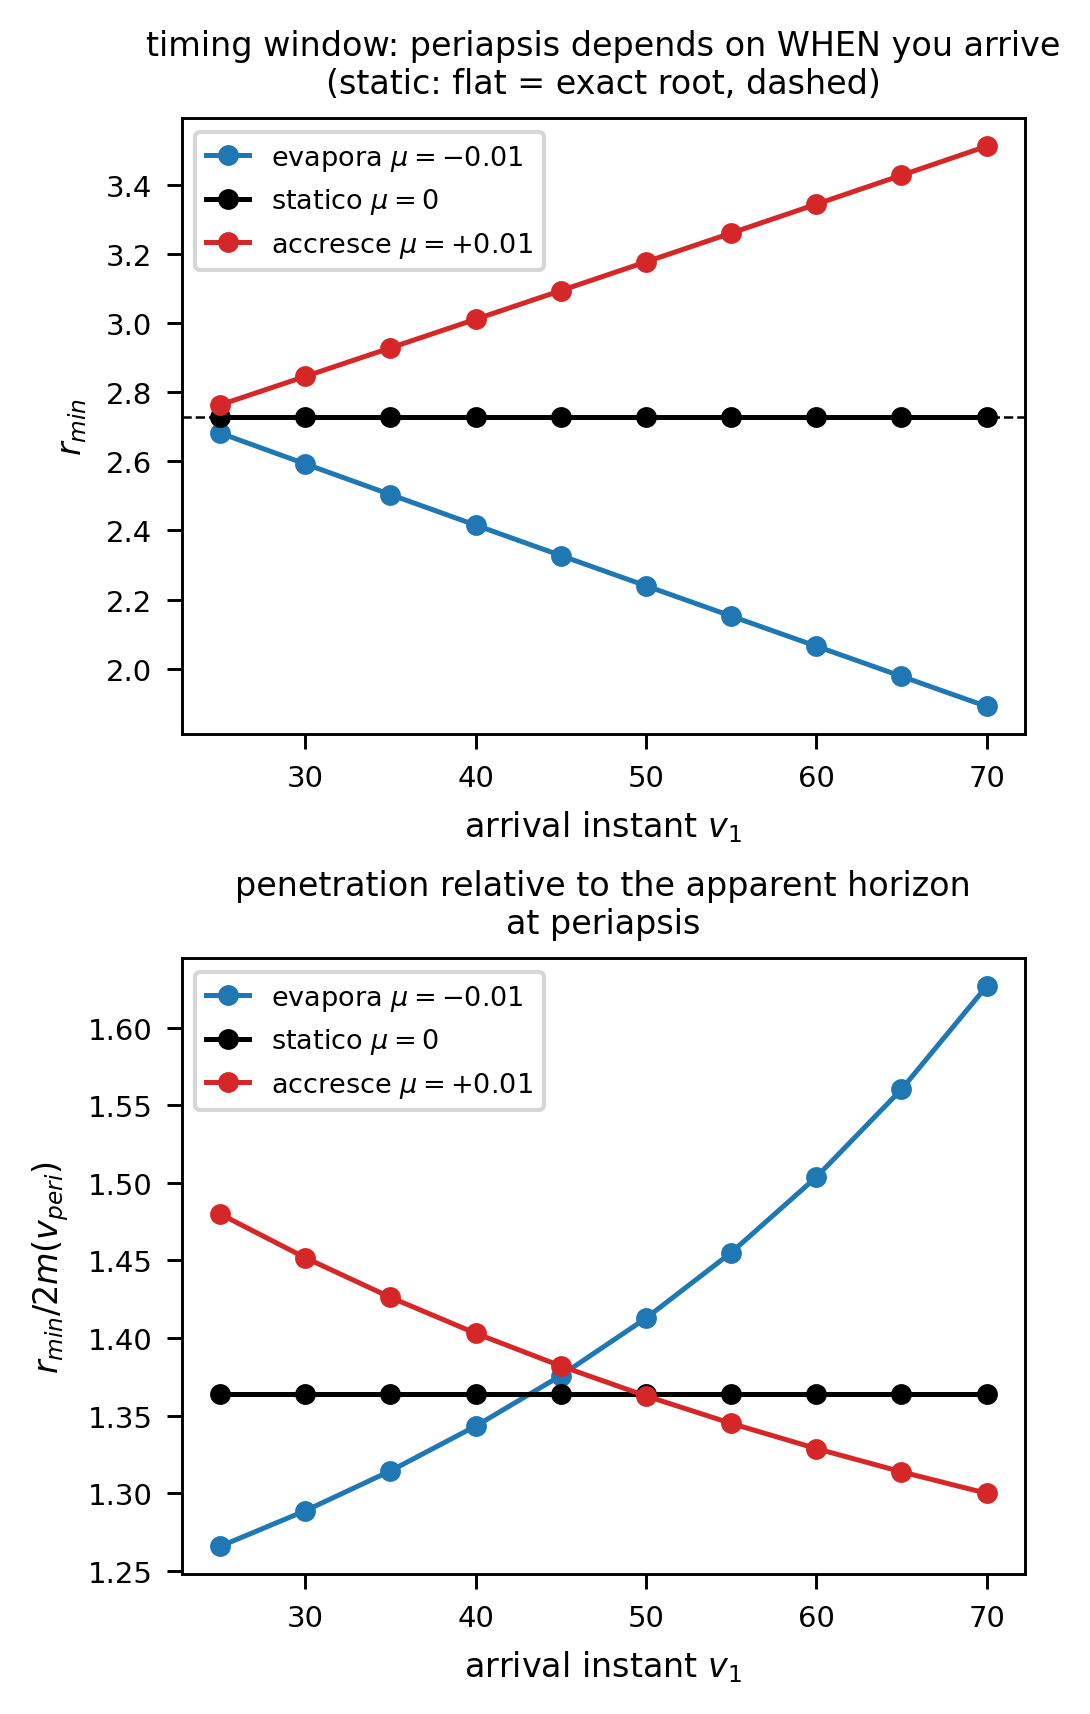
\includegraphics[width=\textwidth,height=0.68\textheight,keepaspectratio]{Immagini/fig_vaidya_timing.png}
    \caption{Timing window: $r_{\min}$ depends on the arrival epoch $v_1$. The
    orbit--horizon race has opposite winners in absolute ($r_{\min}$) and relative
    ($r_{\min}/2m$) terms for accretion vs evaporation.}
    \label{fig:vaidya-timing}
\end{figure}



\bibliographystyle{iopart-num}
\bibliography{refs}

\end{document}
